\chapter{基于传统机器学习方法的低分辨率环境下微表情识别}\label{chap:owner1}

微表情是一种基本的非言语行为,可以忠实地表达人类隐藏的情感。它在国家安全、计算机辅助诊断等领域有着广泛的应用,鼓励我们开展微表情自动识别的研究。然而,从监控视频中获取的图像容易出现质量低下的问题,给实际应用带来困难。由于所捕获图像的质量较低,现有的算法无法达到预期的效果。针对这一问题,我们对面部幻觉法在低分辨率情况下的微表情识别问题进行了全面的研究。实验结果表明,该框架在低分辨率情况下的微表情识别中取得了良好的效果。

目前的微表情识别算法虽然取得了较为合理的效果,但其性能在很大程度上取决于人脸视频剪辑的质量。一旦用于识别的人脸视频片段质量较差(如分辨率较低),上述算法就无法正常工作。原因主要有两个方面:(1)低分辨率图像丢失了大量的细节信息,导致从低分辨率图像序列中提取可用特征的困难\citep{lei2011local}。(2)低分辨率图像与高分辨率图像(如不同分辨率、不同清晰度)不一致,导致我们在测试阶段无法直接使用低分辨率图像作为输入。在现实世界中,从监控录像中获取的面部图像通常只占整个画面的一小部分。例如,用于微表情识别的SMIC数据集的面部分辨率为$190\times230$。然而,监控视频捕捉到的面部图像序列的分辨率往往在$50\times50$(或更低)以下。这意味着以前的微表情识别方法不能直接用于处理低分辨率的情况。因此,低分辨率情况下的微表情识别研究具有重要意义和挑战性。

为了解决上述问题,我们利用最近的面部幻觉方法进行了低分辨率微表情识别的研究。我们首先对低质量的人脸图像序列产生幻觉,以恢复丢失的动态特征。然后,我们采用传统的微表情识别方法来探索低质量的微表情识别。我们评估了不同分辨率下微表情识别准确率的表现,研究了分辨率与识别准确率之间的关系。一般来说,本文的目标是全面研究分辨率对微表情识别的影响,同时开发一个框架来处理低质量条件下的微表情识别任务。

低分辨率微表情识别过程包括图像序列预处理、超分辨率重建、特征提取和分类,如图~\ref{fig10}所示。详细描述如下:

\begin{figure}[!htbp]
    \centering
    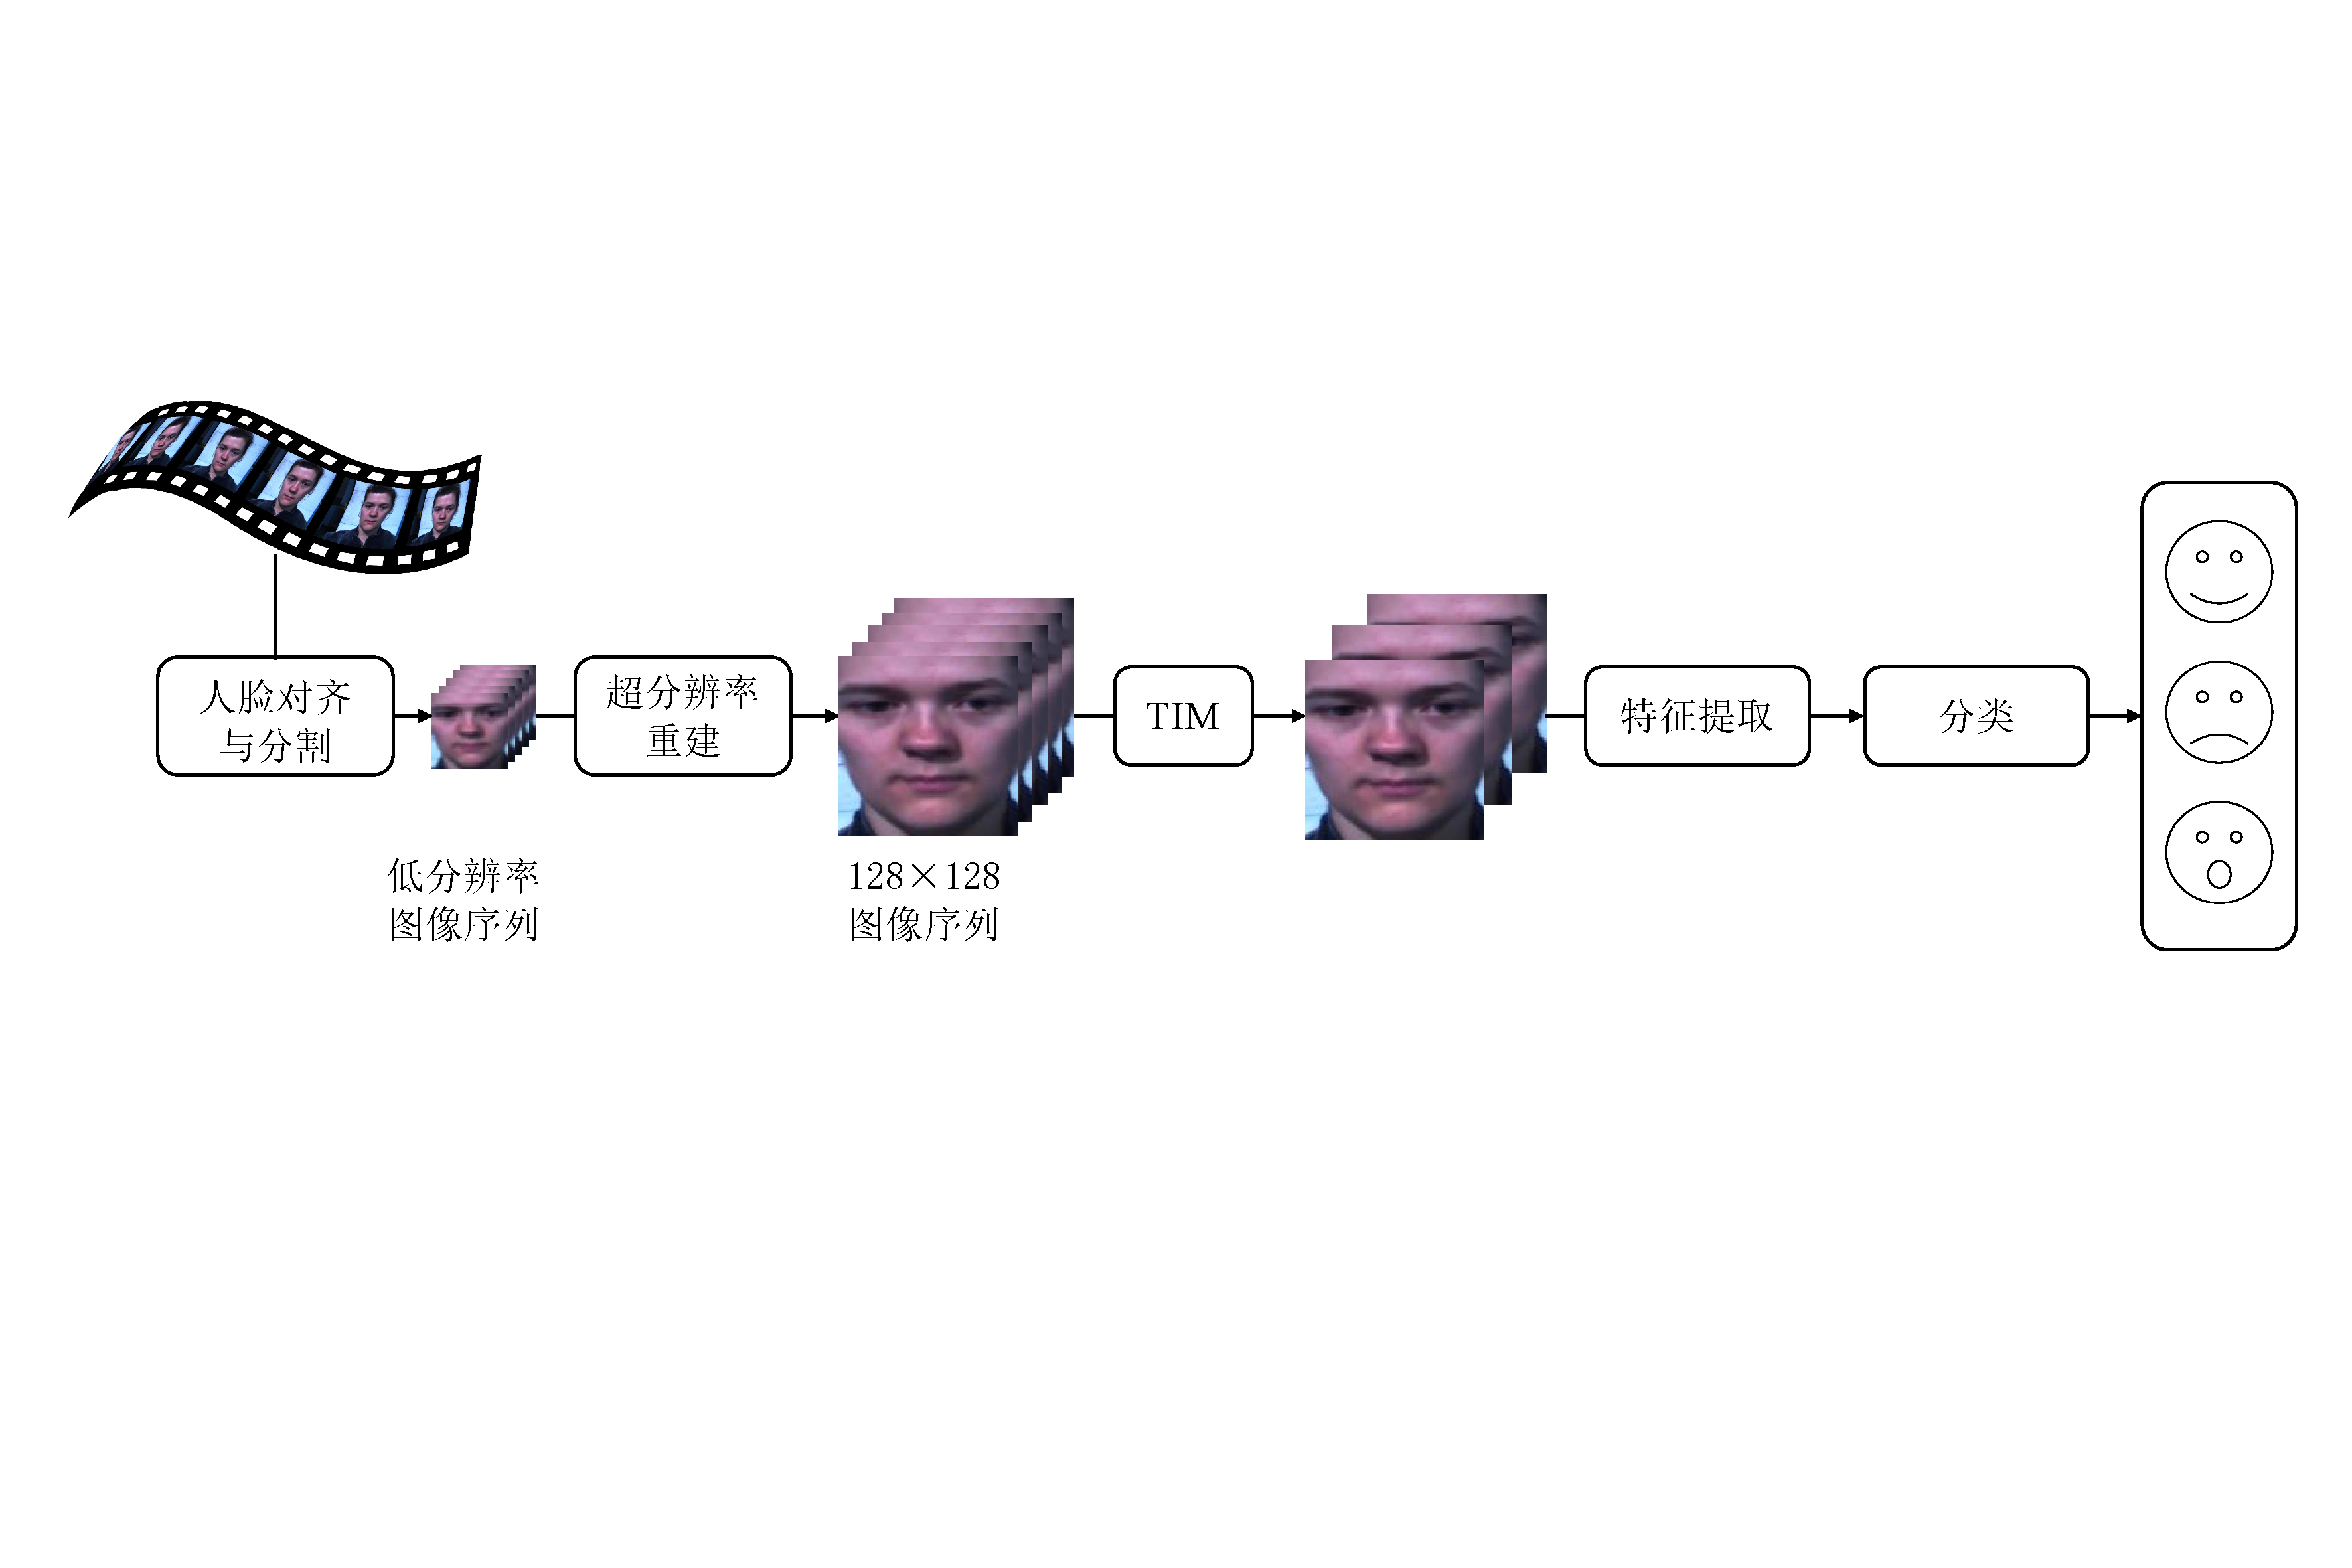
\includegraphics[width=0.95\textwidth]{LR0}
    \caption{低分辨率环境下微表情识别框架}
    \label{fig10}
\end{figure}

\section{低分辨率微表情数据获取}

微表情识别的数据集有很多,如SMIC和CASME II。然而,这些数据集都是专业相机在特定环境下获取的高清图像序列。图~\ref{fig11}显示了SMIC-HS数据集的视频片段中的两帧。我们可以在红色框中发现面部表情的细微变化。特别是白色椭圆区域的运动和白色箭头的位置更为明显。如果图像分辨率太低,这些细节很难被注意到。

\begin{figure}[!htbp]
\centering
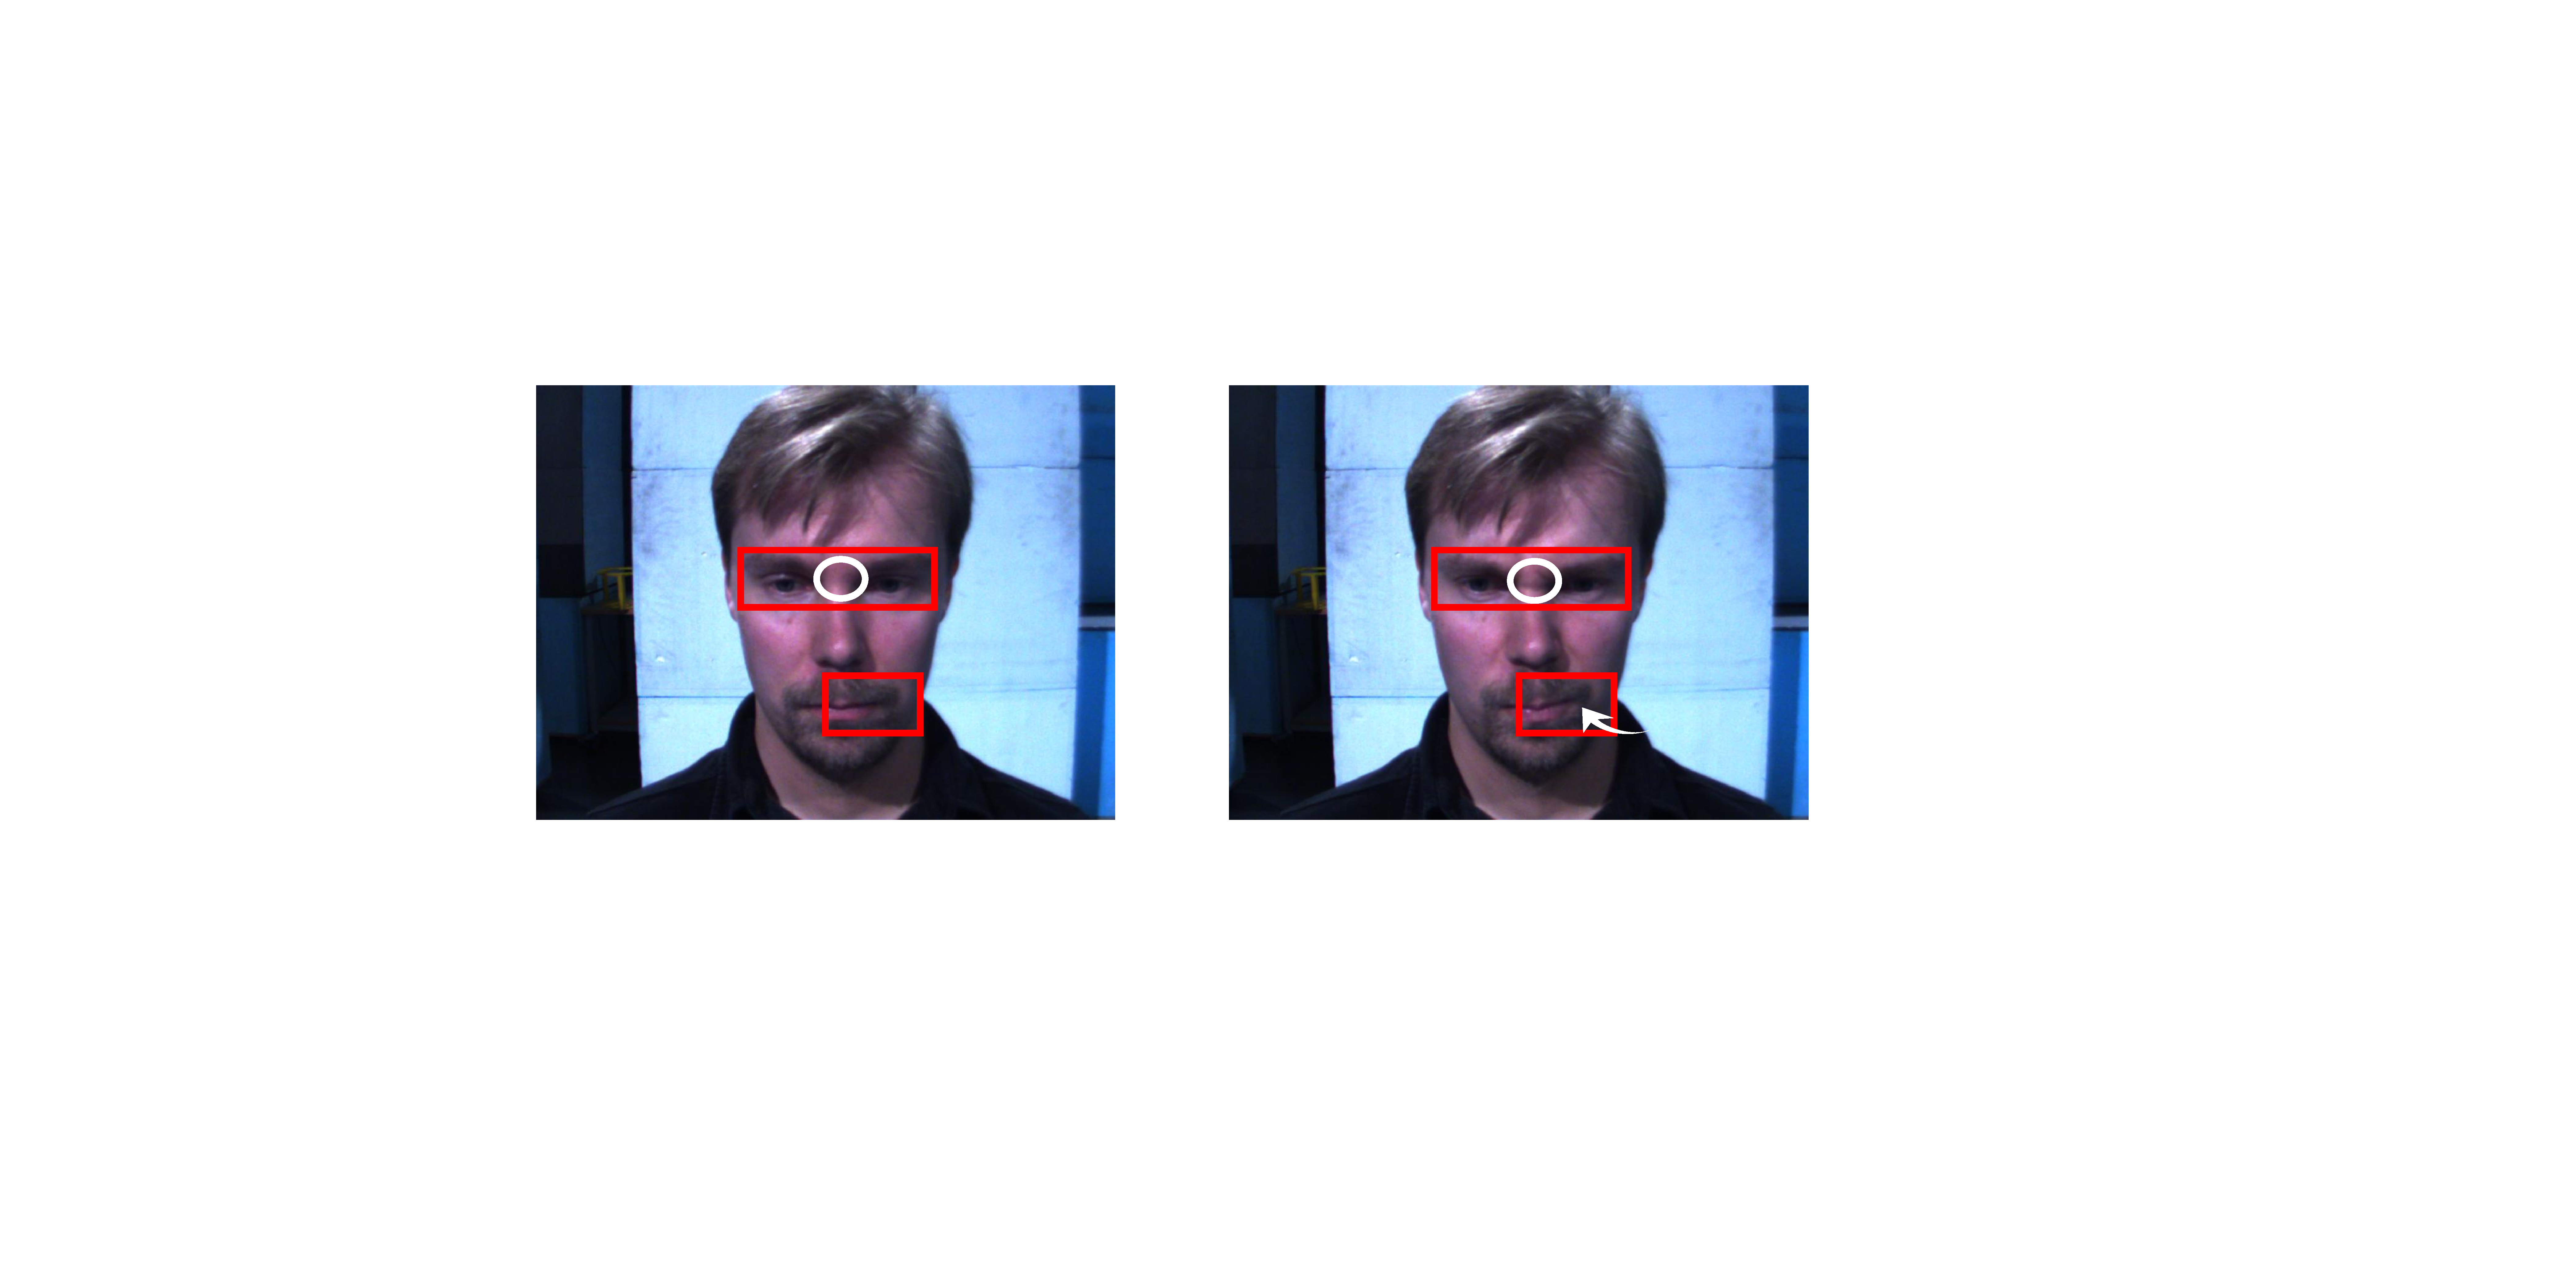
\includegraphics[width=0.65\textwidth]{LR1}
\caption{来自SMIC-HS数据集的两帧}
\label{fig11}
\end{figure}

由于现有的自发微表情数据集中不存在低分辨率的图像序列,我们采用图像恶化处理的方法来获得模拟的低分辨率的微表情图像序列。本文将低分辨率图像分为三大类:小尺寸、低质量和小尺寸放大器、质量较差\citep{wang2014low}。我们考虑第三种类型的图像(小尺寸、质量差),即更接近真实应用的情况,如模拟图像。

在图像重建任务中,低分辨率图像序列是通过对高分辨率图像序列进行模糊、下采样和噪声处理得到的\citep{shi2018hallucinating}:
\begin{equation}
    \label{eq1}
    \boldsymbol{L} = \boldsymbol{DBH}+\boldsymbol{n}
\end{equation}
其中 $\boldsymbol{D}$和$\boldsymbol{B}$分别是下采样和模糊处理,$\boldsymbol{H}$是高分辨率图像,$\boldsymbol{n}$是加性噪声,$\boldsymbol{L}$是低分辨率图像。

\section{数据预处理}

在我们提出的框架中,预处理主要包括三个步骤:人脸对齐、人脸分割和TIM。原始视频中有自然的姿势变化和无意识的运动。同时,收集不同性别、年龄、种族的参与者的微表情视频片段。因此,为了避免上述非表达因子的干扰,进行人脸对齐和人脸分割是必不可少的。

\subsection{主动形状模型}

我们从一个特定的片段中选取一个正面和中性表情的帧作为标准模板,手工定位两只眼睛的位置。然后,利用主动形状模型(Active Shape Model, ASM)检测68个面部地标\citep{cootes1995active}。利用局部加权平均(LWM)建立正则帧68个面部地标与其他帧68个面部地标之间的关系,将微表情图像与正则帧对齐,减少非表情因素的干扰\citep{goshtasby1988image}。

从采集的视频中选取其中没有表情且正面人脸的一帧作为模型脸$\boldsymbol{I_{mod}}$ ,应用ASM算法标定68个人脸关键点$\boldsymbol{\psi(I_{mod})}$,若错误标定其他物品或其他人脸(非主要人脸)时,计算任意对应位置关键点的相对距离$\boldsymbol{L(I_{mod})}$ :
\begin{equation}
    \label{eq2}
    \boldsymbol{L^{(i)}(I_{mod})}=\left \| \boldsymbol{\psi_{I_{mod}}}(p\pm 68)-\boldsymbol{\psi_{I_{mod}}}(q\pm 68) \right \|_{2}^{2\displaystyle }
\end{equation}
其中$i$指标定的关键点组数;$p$、$q$指一个关键点组中任意两点;$n$为关键点的个数,数量为68的倍数。选择相对距离$\boldsymbol{L^{(i)}(I_{mod})}$ 最大的一组关键点确定视频帧中主要人脸。如图~\ref{fig12}所示,1框内为主要人脸,2框为错误识别。

\begin{figure}[!htbp]
\centering
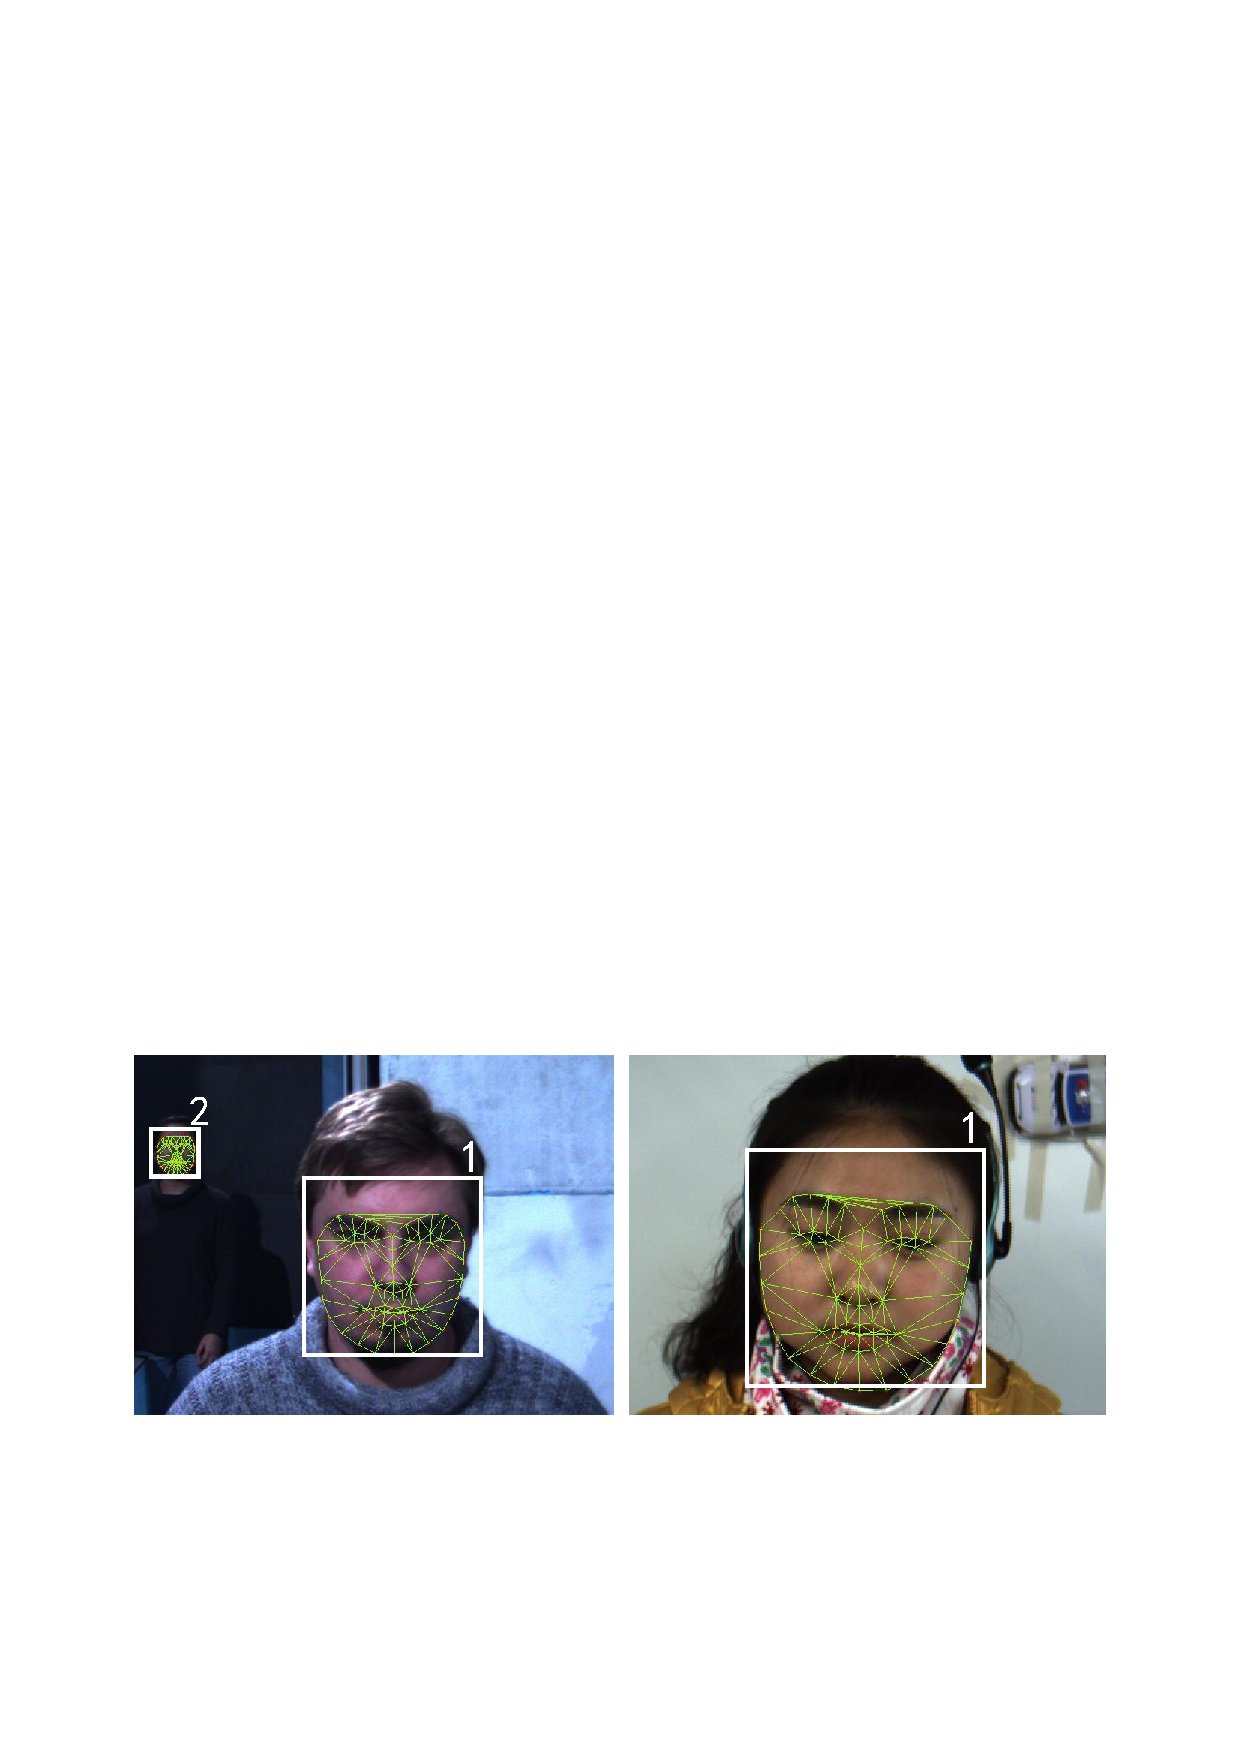
\includegraphics[width=0.65\textwidth]{3LR1}
\caption{ASM算法标定的68个人脸关键点}
\label{fig12}
\end{figure}

\subsection{局部加权平均算法}

对每段个视频的第一帧$\boldsymbol{I_{j,1}}$应用ASM算法标定68个人脸关键点$\boldsymbol{\psi (I_{j,1})}$,使用LWM函数建立模型脸关键点集$\boldsymbol{\psi (I_{mod})}$与视频第一帧关键点集$\boldsymbol{\psi (I_{j,1})}$之间的对应关系:
\begin{equation}
    \label{eq3}
    \boldsymbol{T_{j}}=LWM(\boldsymbol{\psi (I_{mod})},\boldsymbol{\psi (I_{J,1}))},~~j=1,\cdots ,l
\end{equation}
其中$j$是视频段号,$l$是视频片段总数。对视频片段的所有帧应用该关系,使视频的每一帧具有与模型脸$\boldsymbol{\psi (I_{mod})}$统一的姿态:
\begin{equation}
    \label{eq3}
    \boldsymbol{I_{j,k}^{'}}=\boldsymbol{T_{j}}\times \boldsymbol{I_{j,k}},\quad k=1,\cdots ,n_{j}
\end{equation}
其中$\boldsymbol{I_{j,k}}$为第$j$个视频片段的第$k$帧,$\boldsymbol{I_{j,k}^{'}}$为统一姿态后的第$j$个视频片段的第$k$帧,$n_{j}$为$j$视频片段的帧数。如图~\ref{fig13}所示,两图均按照模型脸统一姿态,左图剔除了错误识别,右图改变了头部的倾斜角度。

\begin{figure}[!htbp]
\centering
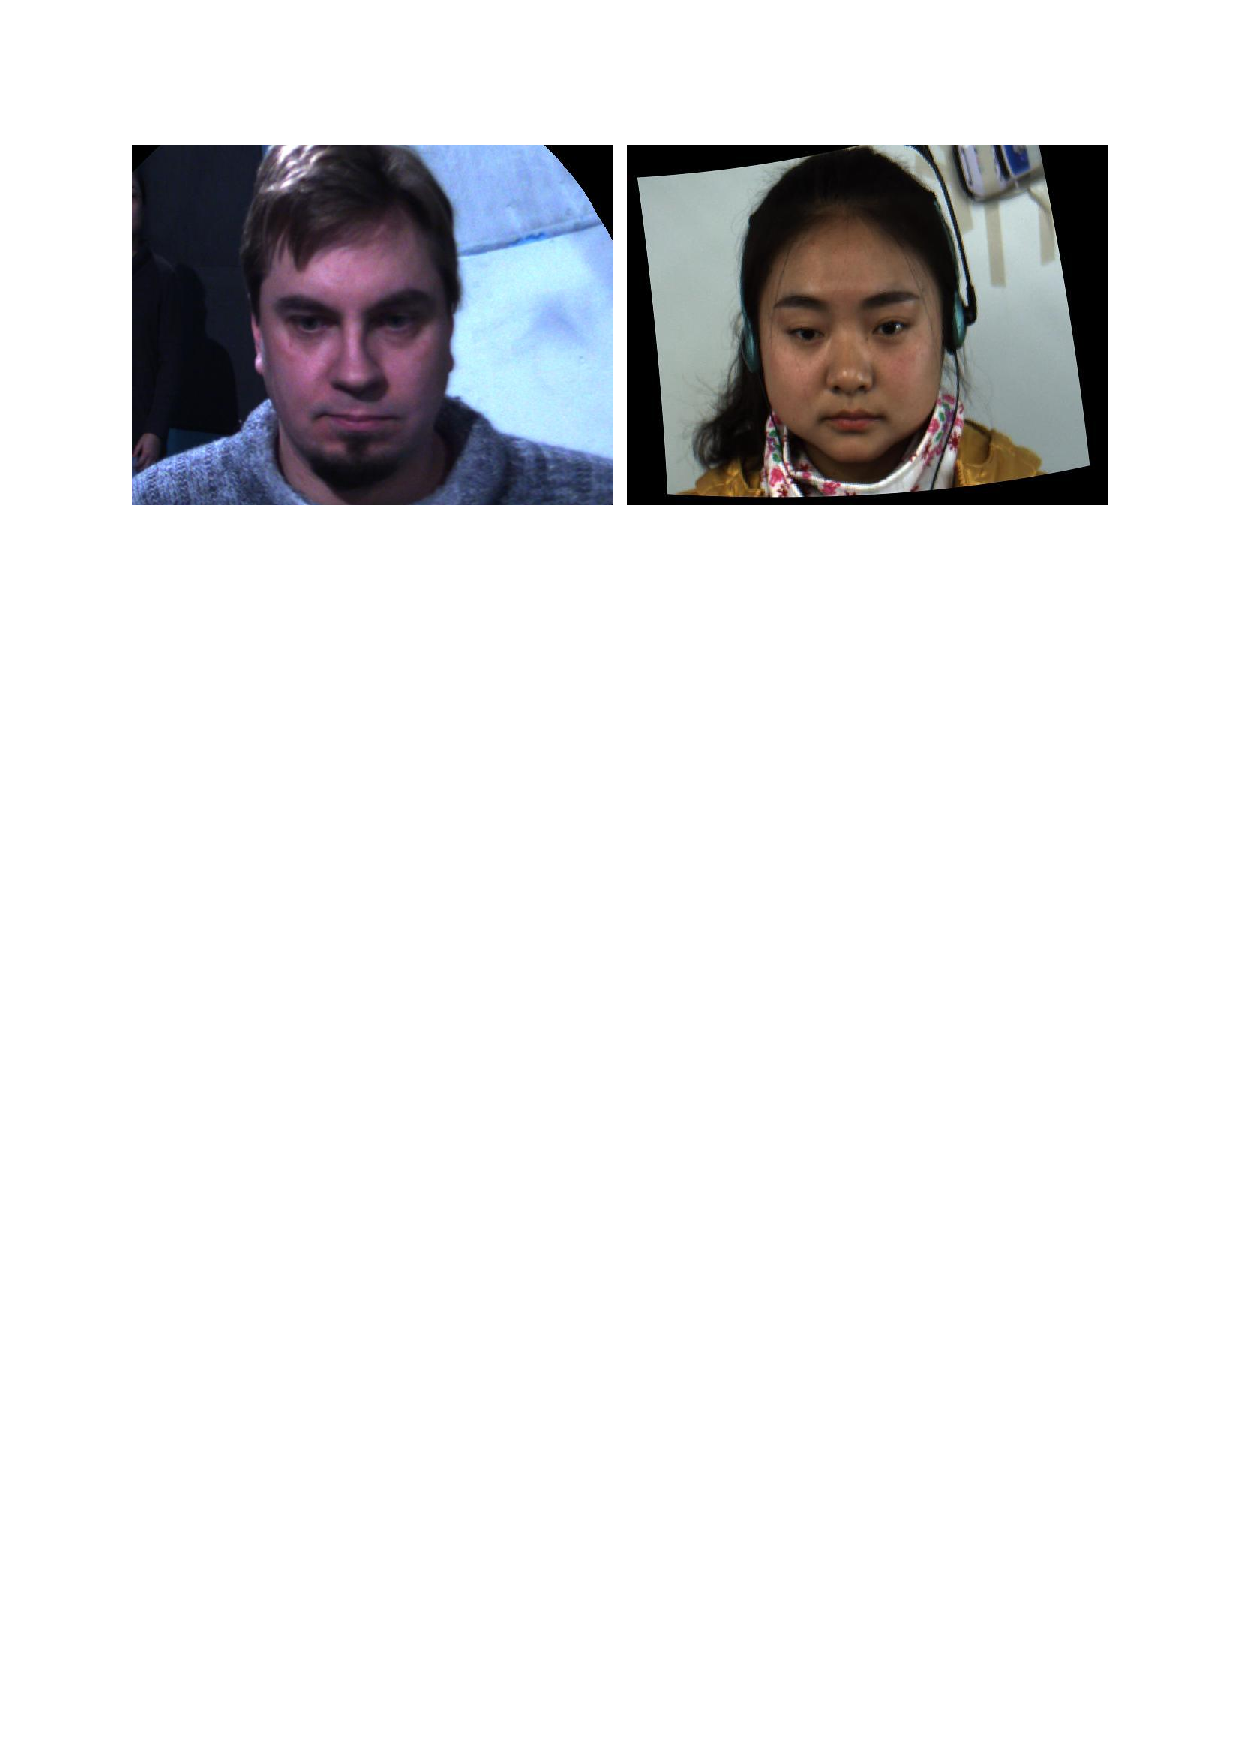
\includegraphics[width=0.65\textwidth]{3LR2}
\caption{LWM算法人脸对齐后的图像}
\label{fig13}
\end{figure}

\subsection{时间插值模型}

微表情视频有不同的长度,从4帧到50帧(如果用100帧/秒的相机拍摄)。为了解决视频片段长度不同的问题,Li等人利用TIM算法将序列的所有帧映射到曲线上,对新合成的人脸图像进行固定间隔采样,最终得到相同的预定义序列长度。实验结果表明,该算法提高了识别精度。图~\ref{fig14}显示了TIM的映射过程\citep{zhou2011towards}。

\begin{figure}[!htbp]
\centering
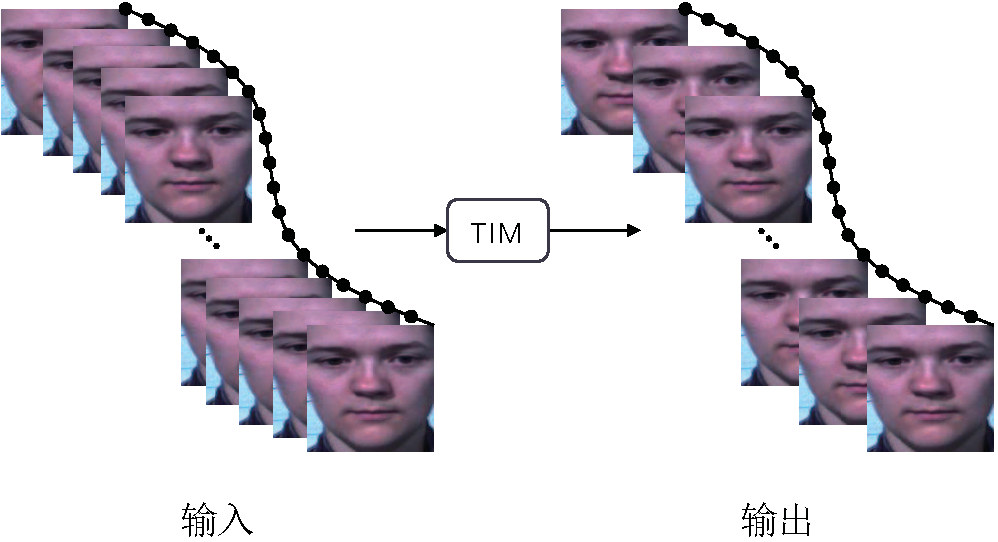
\includegraphics[width=0.65\textwidth]{LR2}
\caption{输入为原始图像序列,输出为TIM算法插值后图像序列}
\label{fig14}
\end{figure}

对由重建出的高分辨率图像组成的图像序列应用TIM算法统一帧数。具体操作为:将重建的图像序列映射到一条非线性曲线上$\mathcal{F}^{n}:\left [ 1/n,1 \right ]\rightarrow \mathbb{R}^{n-1}$ ,
\begin{equation}
    \label{eq4}
    \mathcal{F}^{n}(t)=\begin{bmatrix}f_{1}^{n}(t)\\ f_{2}^{n}(t)\\ \vdots \\ f_{n-1}^{n}(t)\end{bmatrix}
\end{equation}
其中$f_{k}^{n}(t)=sin(\pi kt+\pi (n-k)/n),\quad t\in \left [ 1/n,1 \right ]$ ,$n$为视频段中帧数(图像序列个数),根据实验需求等间距采样,获得统一帧数。

\section{超分辨重建过程}

低分辨率图像和高分辨率图像在质量和分辨率上都是不同的。高分辨率图像序列的微表情识别方法不能直接应用于低分辨率图像序列。在2.1节中,我们介绍了从高分辨率图像生成低分辨率图像的过程。

为了重建高分辨率图像,论文\citepns{shi2018hallucinating}提出了一种新的人脸幻觉算法。将基于块的正则化项与基于像素的正则化项相结合,对目标函数进行约束。重构后的高分辨率图像$\boldsymbol{H}$可以通过最小化以下目标函数得到:
\begin{equation}
 \label{eq4}
 \begin{split}
    f\left ( \boldsymbol{H} \right )= \left \| \boldsymbol{L}-\boldsymbol{DBH} \right \|{_{2}^{2}}+\alpha \boldsymbol{F}_{patch}+\eta \boldsymbol{F}_{pixel}+\lambda \boldsymbol{F}_{penalty}
 \end{split}
\end{equation}
其中右侧第一项为重建误差,后三项分别是基于块的正则项、基于像素的正则项以及惩罚项。图~\ref{fig15}展现了重建工作的具体流程。具体将在下文详细介绍。

\begin{figure}[!htbp]
\centering
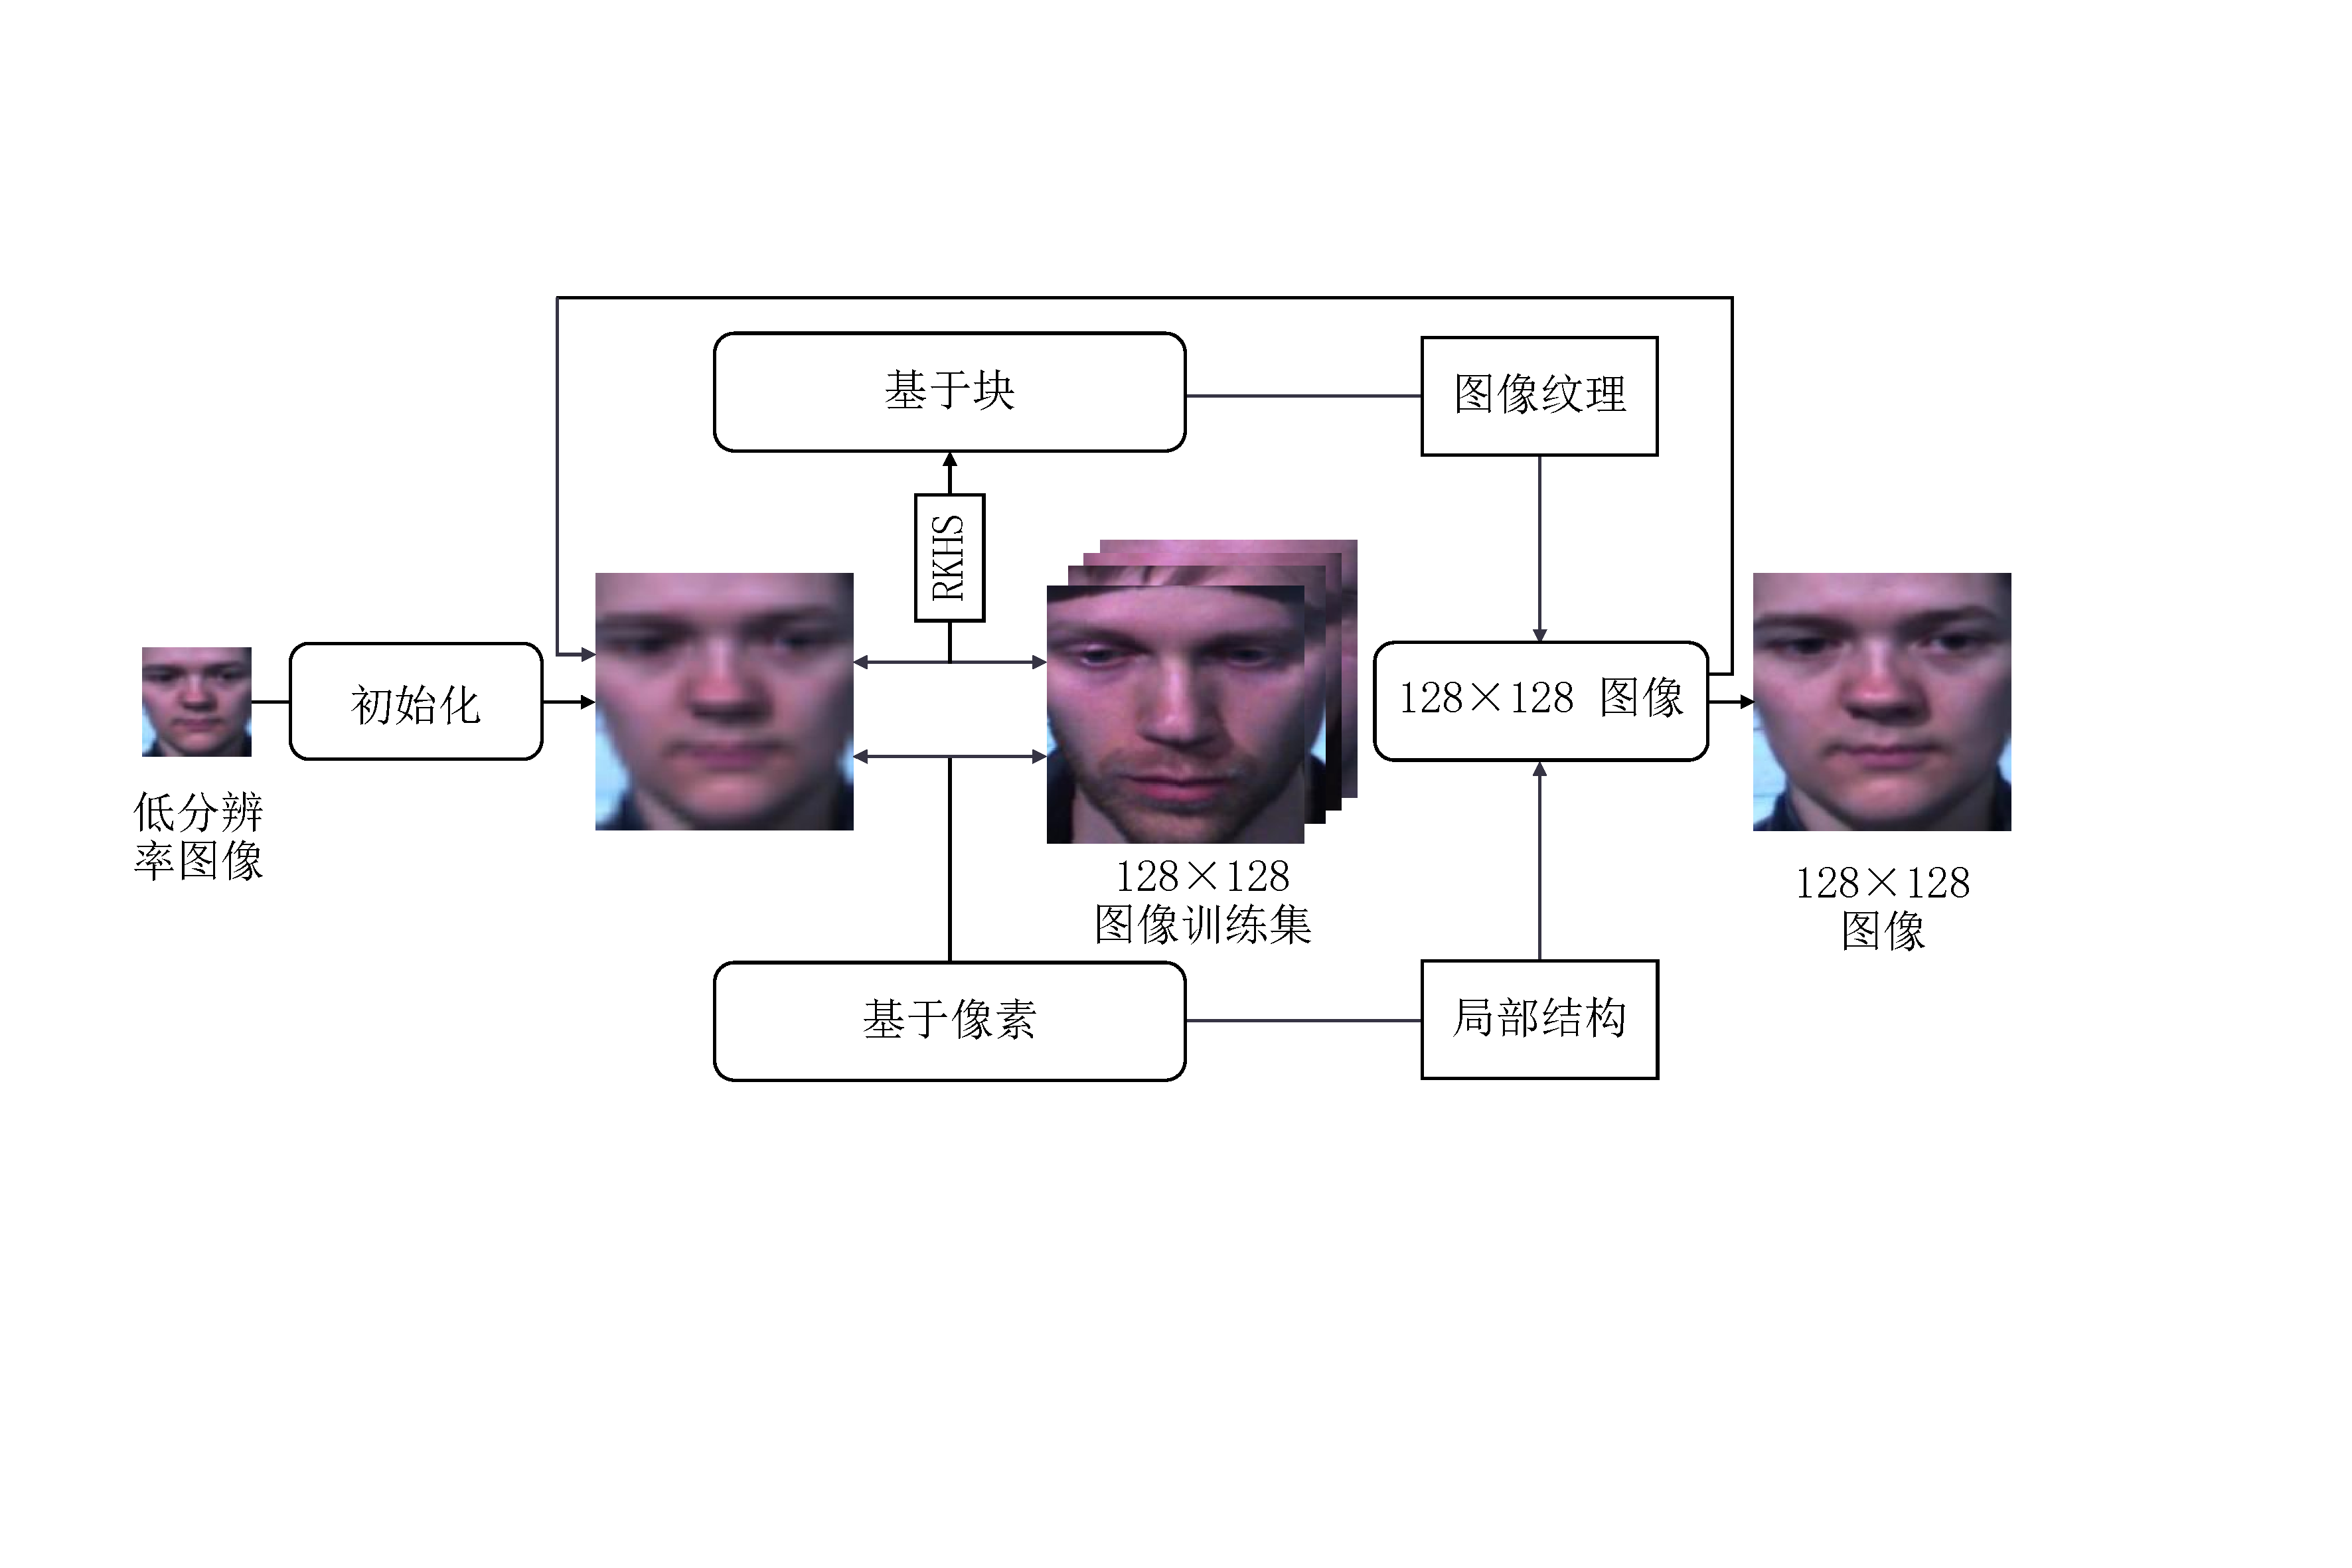
\includegraphics[width=0.75\textwidth]{LR3}
\caption{Super-resolution Reconstruction.}
\label{fig15}
\end{figure}

\subsection{基于的块方法}

将分割后的图像$\boldsymbol{L}$(低分辨率图像)应用三线性插值法调整为与训练样本图像$\boldsymbol{H}$(高分辨率图像,来自公开的高分辨率图像集)大小相等的尺寸,将此图命为$\boldsymbol{H^{(0)}}$(超分辨重建过程的初始图像),对图像分块处理(如分块数为$8\times8$),如图7所示,最小化代价函数:
\begin{equation}
 \label{eq5}
 \begin{split}
   \boldsymbol{J_{\tau }(\omega _{\tau },H^{(k)})} & =\left \{ \left \| \boldsymbol{\phi (R_{\tau }H^{k})}-\boldsymbol{\phi (H_{\tau })\omega _{\tau }} \right \| _{2}^{2}+\boldsymbol{\lambda} \left \| \boldsymbol{d_{\tau }}\bigotimes \boldsymbol{\omega _{\tau }} \right \|_{2}^{2}\right \} \\
   \boldsymbol{s.t. 1^{T}\omega _{\tau }}= 1 & ,2,\cdots ,M
 \end{split}
\end{equation}
估算结合系数$\boldsymbol{\omega _{\tau }}$ ,将其初始结合系数命名为$\boldsymbol{\omega_{\tau }^{0}}$,此时$\boldsymbol{H^{(k)}}$ 已知,即$\boldsymbol{H^{(0)}}$ ,其中$\boldsymbol{\tau}$为图像中图像块的位置,$\boldsymbol{R_{\tau }}$为提取所有图像集位置$\tau$的图像块的矩阵, $\boldsymbol{H_{\tau }}=\left [ h_{\tau }^{1},\cdots ,h_{\tau }^{N} \right ]$为高分辨率图像位置$\boldsymbol{\tau}$处图像块集($N$为训练样本的数量,即高分辨率图像集的数量),$\boldsymbol{\phi (\cdot )}$ 为从原始空间到无限维再生核希尔 伯特空间(Reproducing Kernel Hilbert Space, RKHS)的映射,$\boldsymbol{d_{p}}$ 描述了目标高分辨率块(重建出的块)与相应的训练样本块在核映射空间的核相似性,$\bigotimes$ 表示哈达玛积,$\boldsymbol{\lambda}$为惩罚参数,$\boldsymbol{1}$为全为1的列向量,$M$为图像的块数。

将获得的$\boldsymbol{\omega _{\tau }}$($\boldsymbol{\omega_{\tau }^{0}}$)代入公式(5),并最小化:
\begin{equation}
 \label{eq6}
 \begin{split}
   \boldsymbol{f(H)}= \left \| \boldsymbol{L^{k}}-\boldsymbol{DBH^{k}} \right \|_{2}^{2}+\boldsymbol{\eta \sum_{\tau }}\left \| \boldsymbol{x_{\tau }h^{k}}-\boldsymbol{\beta _{\tau }H_{\tau }} \right \|_{2}^{2}+ \\
   \boldsymbol{\alpha \sum_{\tau }}(\left \| \boldsymbol{\phi (R_{\tau }H^{k})}-\boldsymbol{\phi (H_{\tau })\omega _{\tau } }\right \|_{2}^{2}+ \boldsymbol{\lambda} & \left \| \boldsymbol{d_{\tau }}\bigotimes \boldsymbol{\omega _{\tau } }\right \|_{2}^{2})+\boldsymbol{\sigma MSE} \\
   \boldsymbol{s.t. \quad 1^{T}\omega _{\tau }}= 1,2,\cdots ,M \qquad \qquad \qquad \qquad \qquad \quad &
 \end{split}
\end{equation}
获得重建的高分辨率图像$\boldsymbol{H^{(k)}}$(初始结果命名为$\boldsymbol{H^{(1)}}$),其中$\boldsymbol{D}$为下采样矩阵,$\boldsymbol{B}$为模糊处理矩阵,$\boldsymbol{\beta _{\tau }}$为规范全局优化的像素间关系矩阵,$\boldsymbol{MSE}$为均方误差,$\boldsymbol{\eta }$为基于像素正则项的权重,$\boldsymbol{\alpha}$为基于块正则项的权重,$\boldsymbol{\sigma}$为均方误差的权重。
% \subsection{基于像素的方法}


\section{微表情识别}
如图~\ref{fig10}所示,微表情识别主要分为两部分:特征提取和分类。在以往的微表达分析方法中研究人员展示了LBP-TOP及其变体作为特征描述符的优势。与传统的基于单个图像的LBP特征不同,LBP-TOP可以捕捉到空间和时间域的动态变化,这对于微表情识别是必不可少的。我们首先将整个人脸图像序列划分为几个长方体,如$ 5\times5\times1 $,$ 8\times8\times2 $等,其中前两个参数决定了空间域中的块数,最后一个参数是时间方向上的段数。每个长方体都可以看作一个新的单位。LBP特征提取自新单元中三个不同的正交平面(XY、XT、YT)。我们遍历所有长方体,得到图像序列的LBP-TOP特征,然后将每个长方体的LBP-TOP特征串联起来。如图5所示。

在分类部分,我们使用线性支持向量机(LSVM)作为分类器\citep{chang2011libsvm}。为了进行公平的比较,我们在实验中采用了一主体退出协议。根据数据集发布方提供的微表情表签,我们将来自SMIC的样本分为三类(positive, negative, surprise),来自CASME II的样本分为五类(happiness, surprise, repression,disgust, and other)。

% \subsection{LBP-TOP特征提取}



\subsection{LSVM}

支持向量机(Support Vector Machine, SVM)是曾经打败神经网络的分类方法,从90年代后期开始在很多领域均有举足轻重的应用,近年来,由于深度学习的兴起,SVM的风光开始衰退,但是其仍然不失为一种经典的分类方法。SVM最初由 Vladimir N. Vapnik 和 Alexey Ya. Chervonenkis于1963年提出,之后经过一系列改进,现今普遍使用的版本由Corinna Cortes 和 Vapnik于1993年提出,并在1995年发表。深度学习兴起之前,SVM被认为是机器学习近几十年来最成功、表现最好的方法。

本文讨论线性可分的支持向量机,详细推导其最大间隔和对偶问题的原理。简单起见,以二分类为例,如下图,设训练集为D={(x1,y1),...,(xn,yn)}D={(x1,y1),...,(xn,yn)},蓝色圆点为一类,红色方块为另一类,分类的目标是寻找一个超平面,将两类数据分开。在二维平面中,分类超平面就是一条直线,从图中可以看出,能将训练样本分开的超平面有很多可能(图中绿色虚线),超平面除了要将训练集中的数据分开,还要有较好的泛化性能,需要把测试集中的数据也划分开。从直观上看,绿色实线是比较好的一个划分,因为该直线距离两类数据点均较远,对于数据局部扰动的容忍性较好,能够以较大的置信度将数据进行分类。


\section{实验及分析}

我们现在在三个不同的自发微表达数据集上展示实验和结果,即SMIC-HS, SMIC-subHS和CASME II。实验参数的设置和结果分析将在下面的小节中讨论。

\begin{table}[!htbp]
\centering
\caption{实验中使用的数据集}
\label{tab4}
\begin{tabular}{c|ccc}
\hline
 & SMIC-HS & SMIC-subHS & CASME II \\ \hline
微表情数 & 164 & 71 & 247 \\
参与者 & 16 & 8 & 26 \\
分类 & 3 & 3 & 5 \\ \hline
\end{tabular}
\end{table}

SMIC- hs和SMIC- subhs是SMIC的两个子集。SMIC-HS数据集包含来自16名参与者的164个自发微表情片段,分为三类:阳性(51个片段)、阴性(70个片段)和惊奇(43个片段)。SMIC-subHS数据集是SMIC-HS的子集,只包含最后8个参与者。前8名受试者的微表达片段数量差异较大,其中3名受试者贡献了整个组近一半的微表达样本,这可能会影响“一受试者退出”的表现,而后8名受试者的s (SMIC-subHS)片段数量分布较为均匀。SMIC-subHS数据集中,正负、惊喜片段分别为28、23、20个。同时,CASME II数据集包含26名参与者,分别属于5个不同的类别:惊讶(25个片段)、幸福(32个片段)、其他(99个片段)、厌恶(64个片段)和压抑(27个片段)。表1显示了实验中使用的数据集的摘要。面部高分辨率图像的分辨率设置为$ 128 \times 128 $的实验。$ 128 \times 128 $分辨率的图像下采样乘以2,4,8次获得低分辨率图像(如图6)。这意味着我们评估三个不同层次的低分辨率的面部图像序列(如$ 16 \times 16 $, $ 32 \times 32 $, $ 64 \times 64 $)的微识别任务。

\begin{figure}[!htbp]
    \centering
    \begin{subfigure}[b]{0.35\textwidth}
      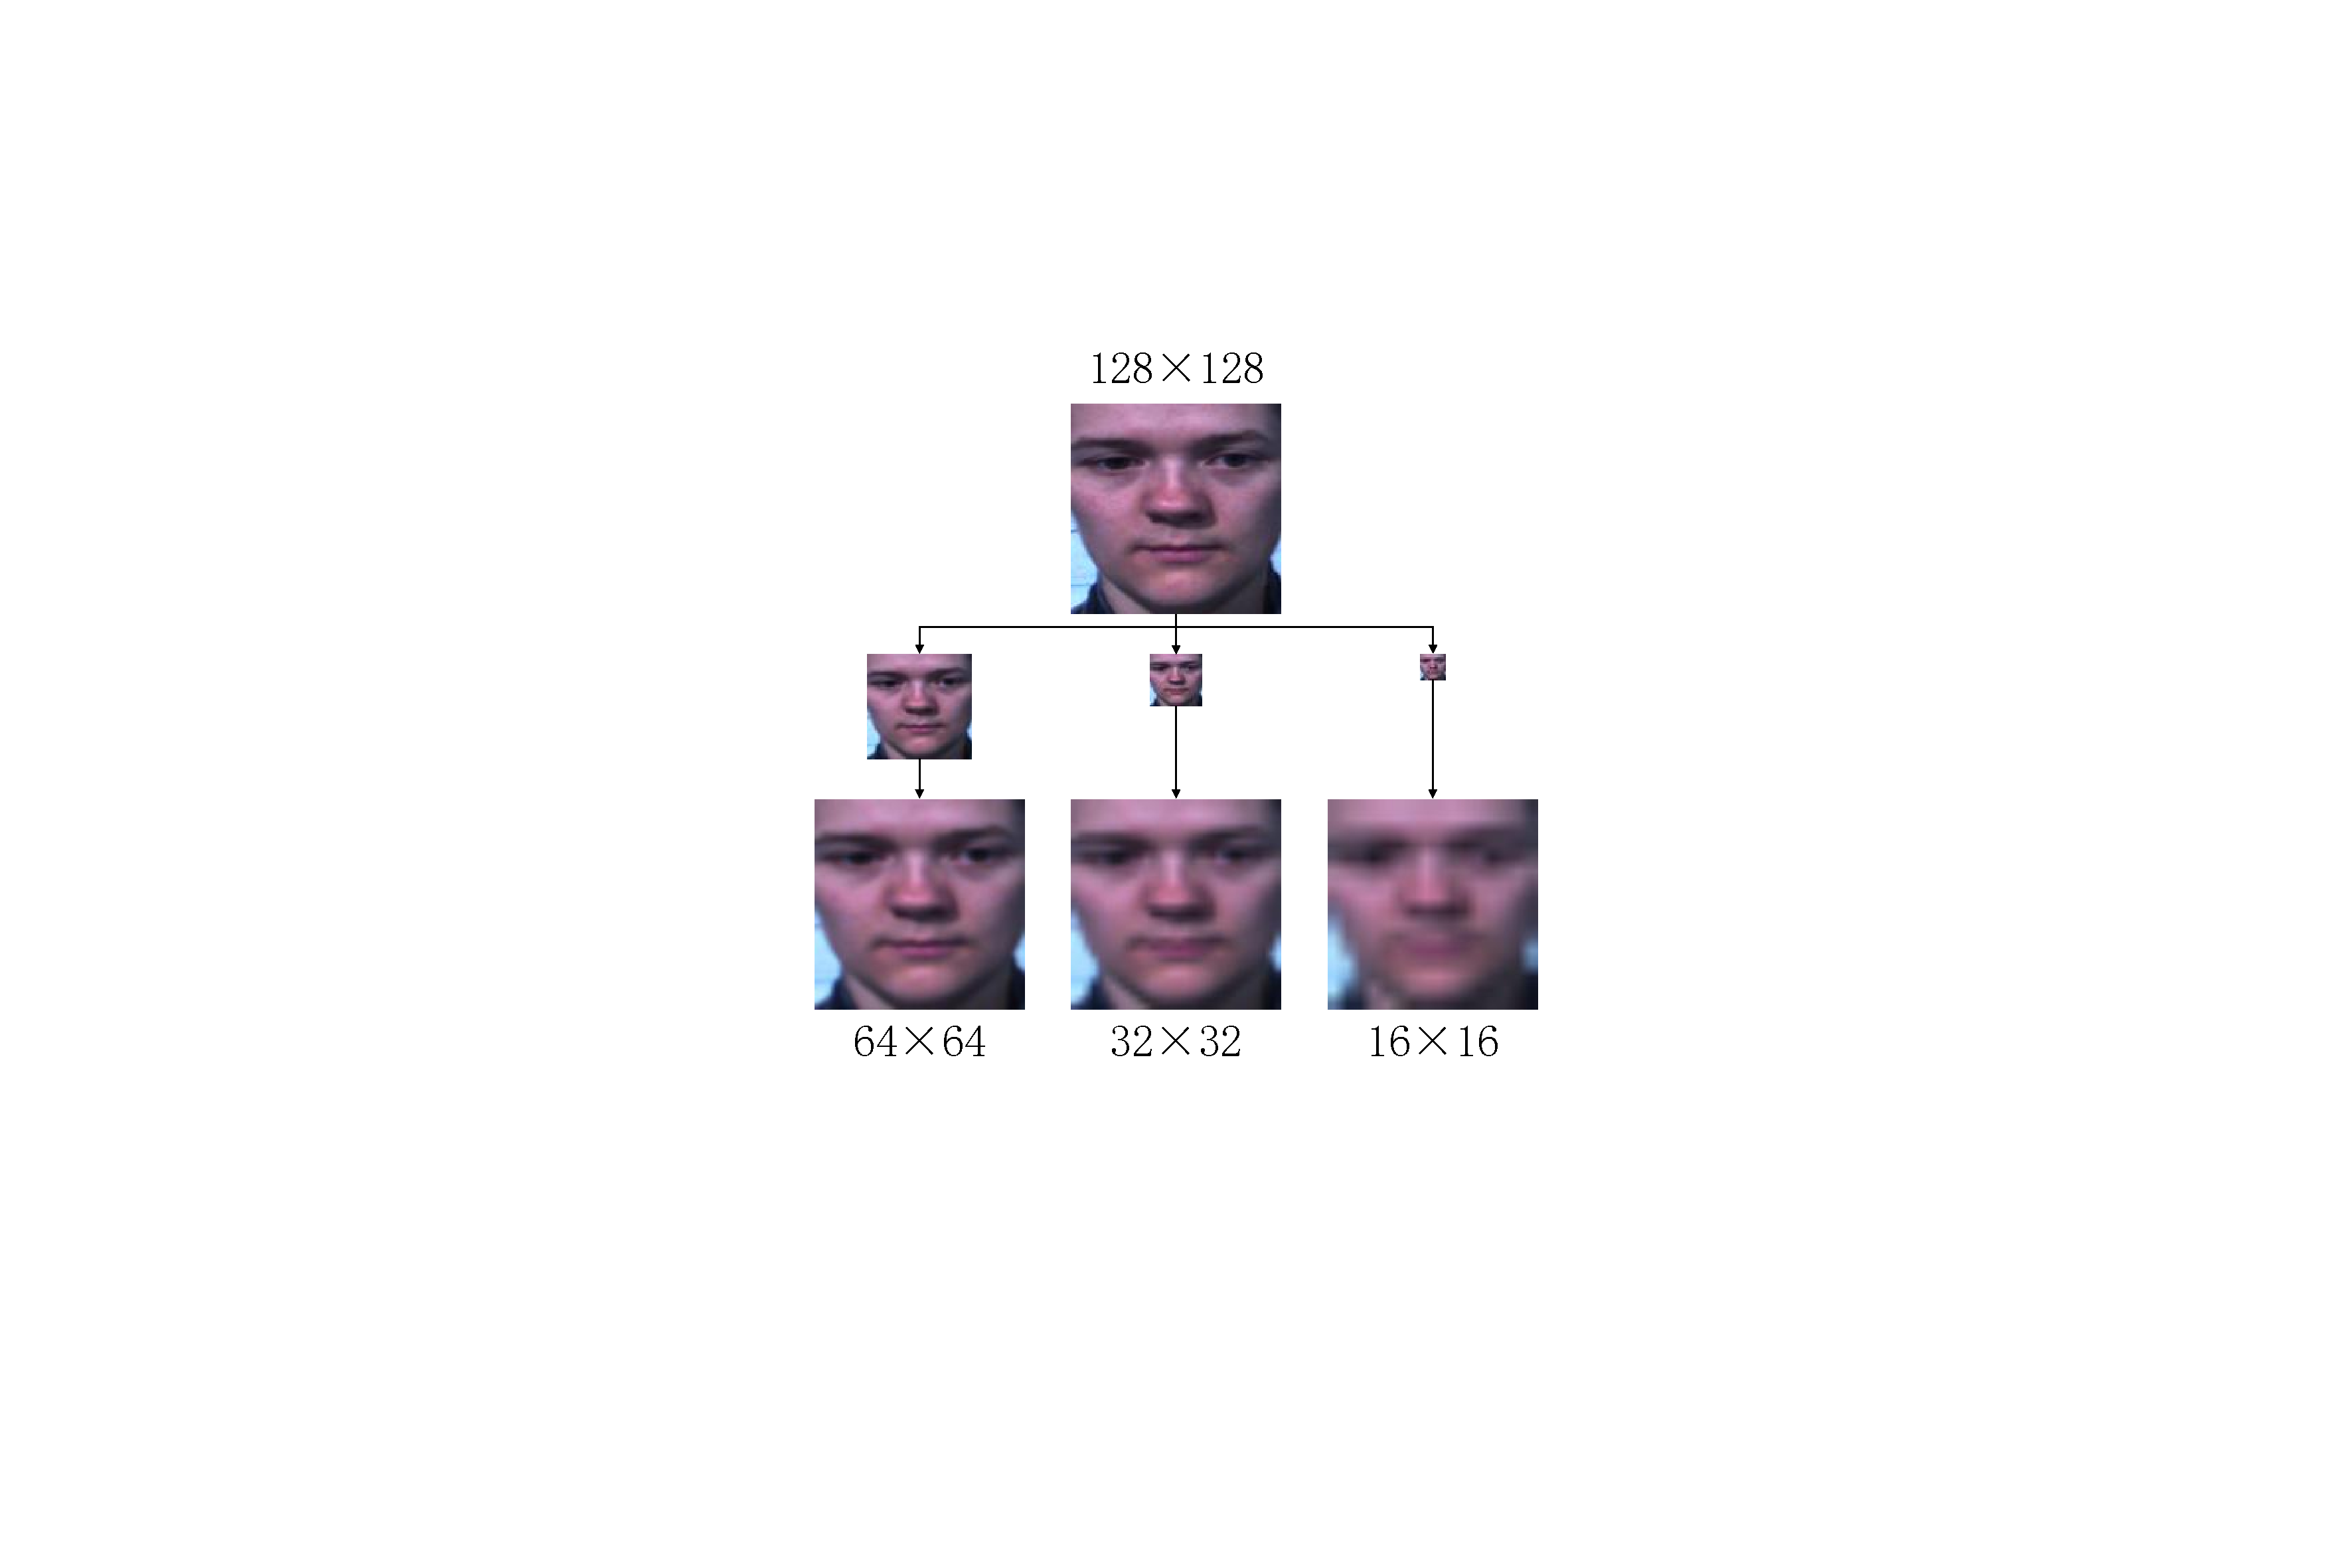
\includegraphics[width=\textwidth]{LR41}
      \caption{}
    \end{subfigure}%
    ~ ~%add desired spacing
    \begin{subfigure}[b]{0.35\textwidth}
      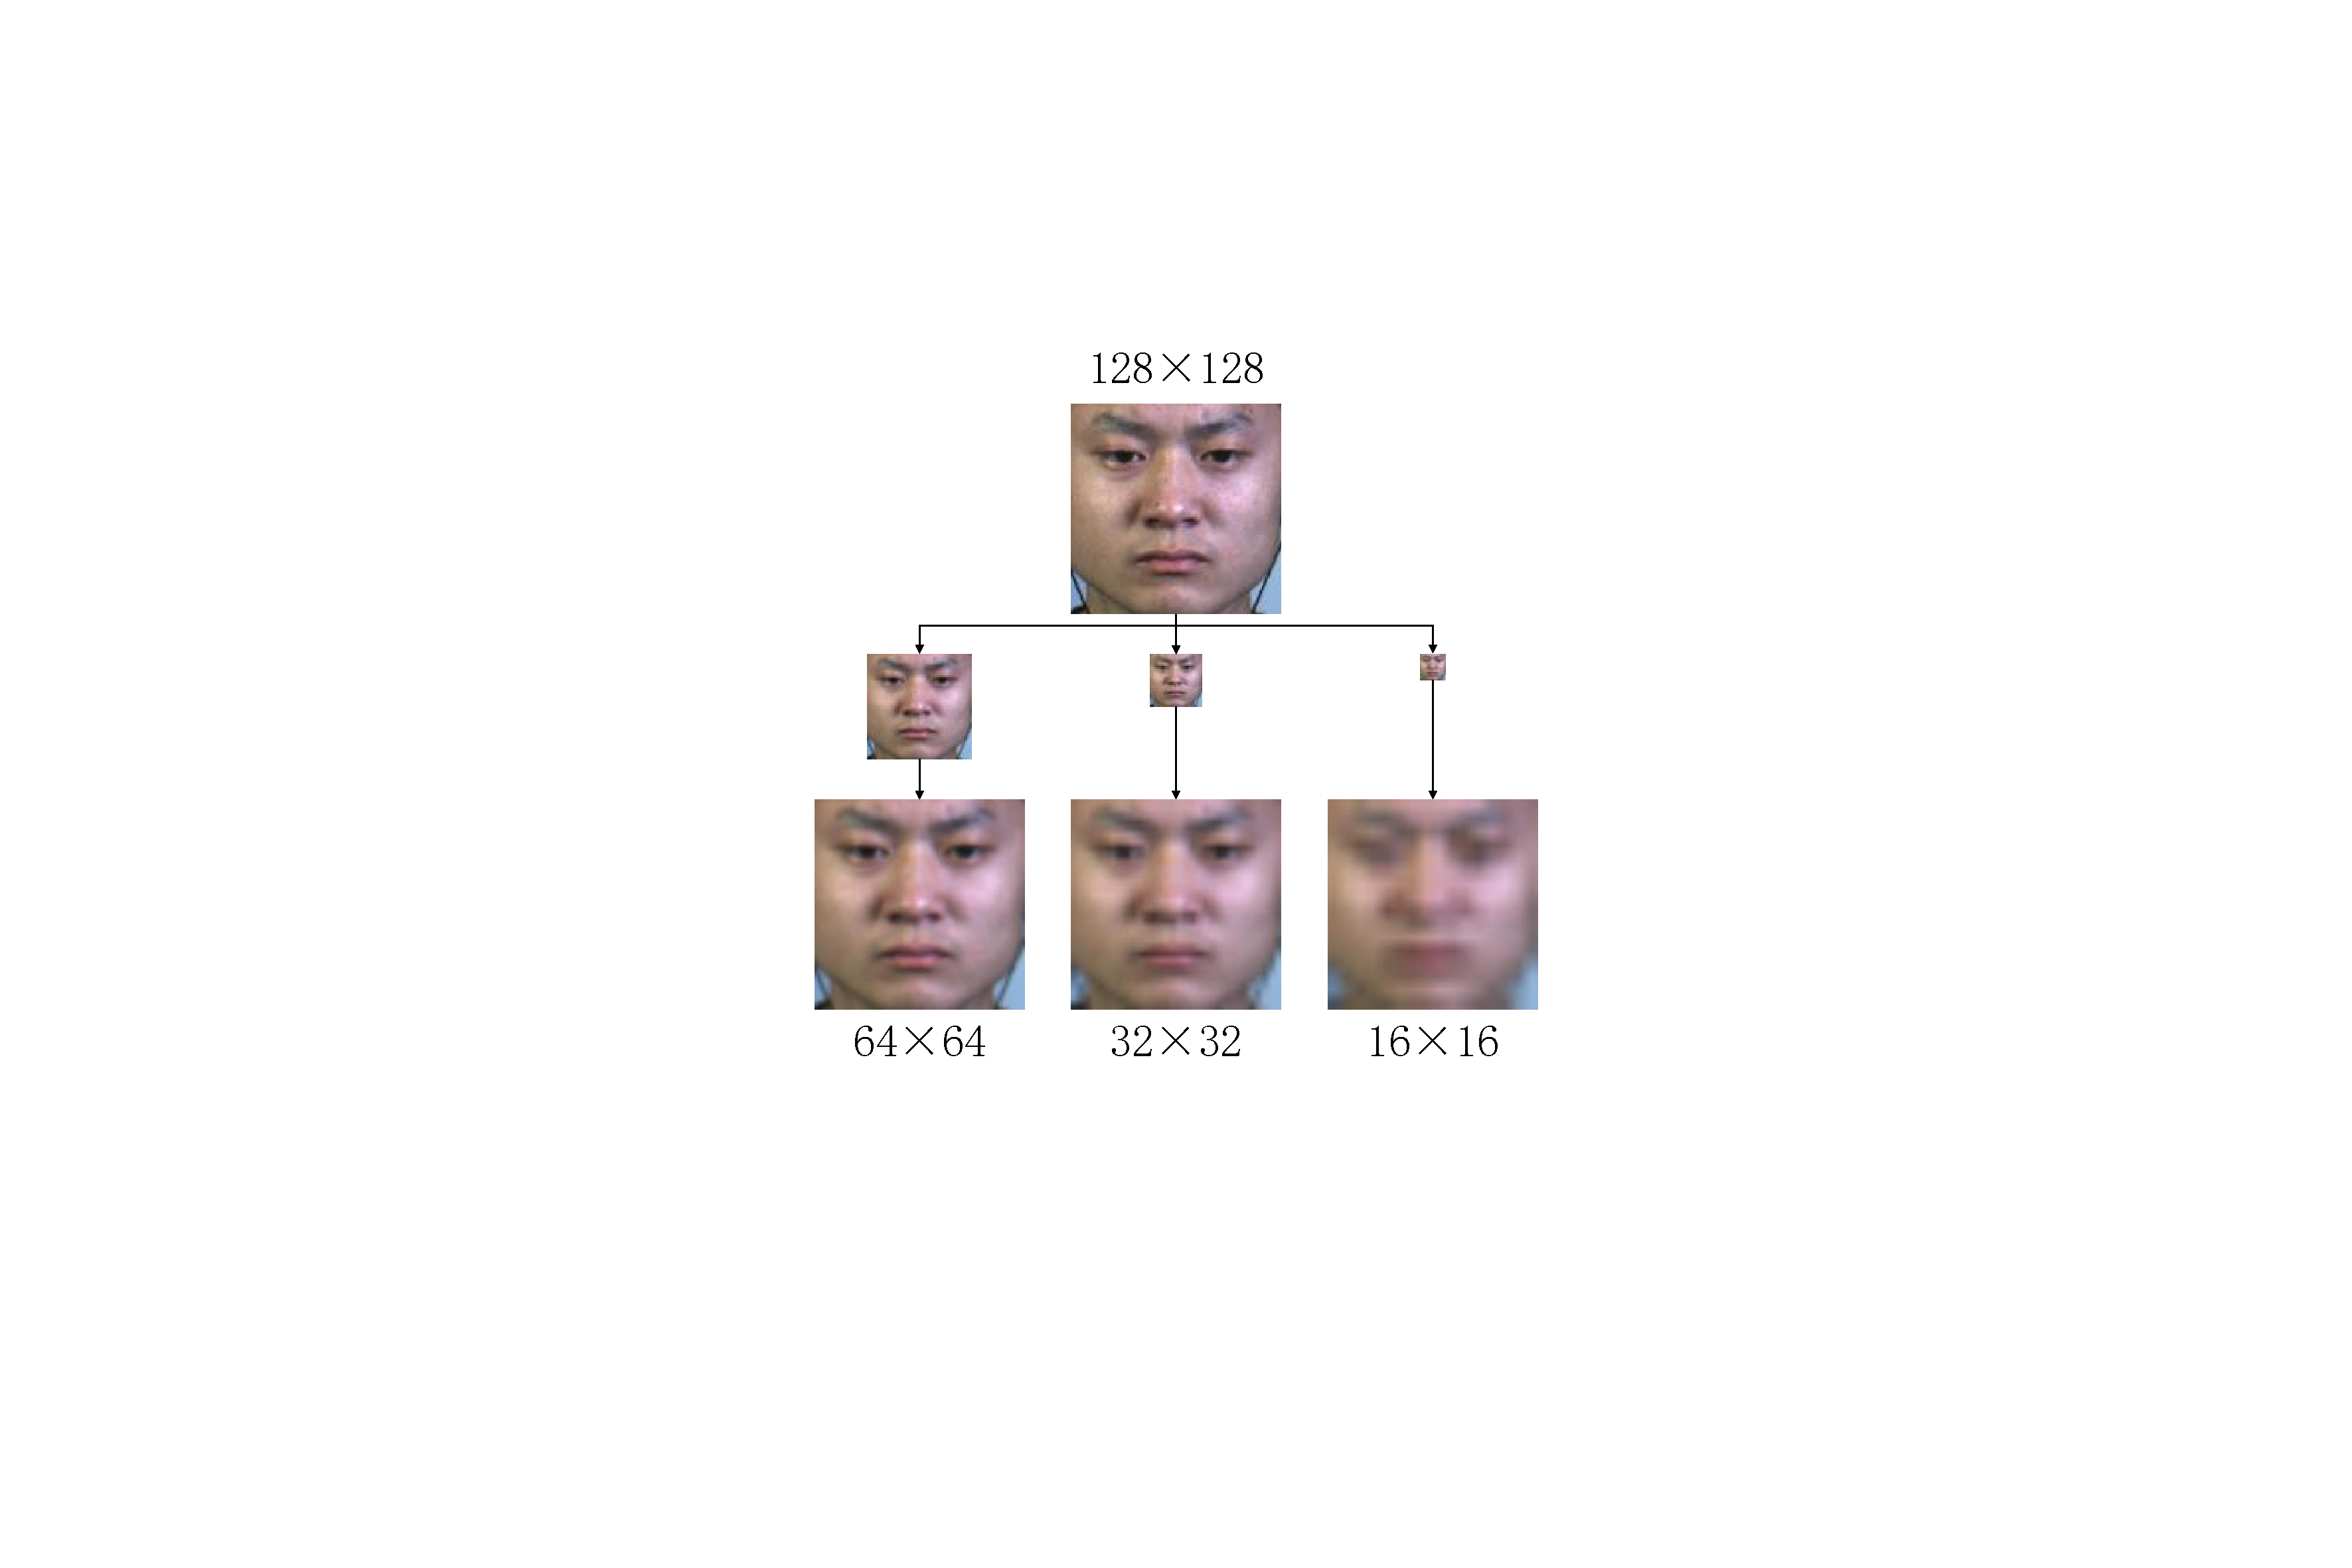
\includegraphics[width=\textwidth]{LR42}
      \caption{}
    \end{subfigure}
    \caption{低分辨率图像\\ \footnotesize \textmd{(a) SMIC-HS/SMIC-subHS数据集低分辨率图像,(b) CASME II数据集低分辨率图像}}
    \label{fig14}
\end{figure}

在本节中,利用论文\citepns{shi2018hallucinating}提出的方法将低分辨率图像重建为高分辨率图像,该方法在2.3节中进行了简要介绍。表2-3列出了不同分辨率下重建图像序列的平均峰值信噪比(PSNR)和结构相似度(SSIM)指数。在这里,我们分别使用S64、S32和S16来命名分辨率为$ 64 \times 64 $, $ 32 \times 32 $和$ 16 \times 16 $的重建图像序列。

\begin{table}[!htbp]
\centering
\caption{重建图像序列的平均PSNR(dB)指标}
\label{tab5}
\begin{tabular}{c|ccc}
\hline
PSNR (dB) & $ 16 \times 16 $ & $ 32 \times 32 $ & $ 64 \times 64 $ \\ \hline
SMIC-HS & 31.25 & 37.67 & 44.30 \\
SMIC-subHS & 31.67 & 38.26 & 43.22 \\
CASME II & 31.80 & 36.49 & 37.83 \\ \hline
\end{tabular}
\end{table}

\begin{table}[!htbp]
\centering
\caption{重建图像序列的平均SSIM指标}
\label{tab6}
\begin{tabular}{c|ccc}
\hline
SSIM & $ 16 \times 16 $ & $ 32 \times 32 $ & $ 64 \times 64 $ \\ \hline
SMIC-HS & 0.9397 & 0.9775 & 0.9883 \\
SMIC-subHS & 0.8970 & 0.9346 & 0.9424 \\
CASME II & 0.9439 & 0.9761 & 0.9882 \\ \hline
\end{tabular}
\end{table}

如表2和表3所示,重建的人脸图像序列的定量指标(PSNR/SSIM)与输入人脸图像序列的分辨率成正比。例如,在SMIC-HS数据集中,S16的PSNR指数为31.25dB,比S32低6.42dB,比S64低13.05dB。对于SSIM指数,S16达到0.9397,比S32低0.0378,比S64低0.0486。此外,图7给出了重建后的图像序列的视觉表现,也表明了与上述观点相同的结论。

\begin{figure}[!htbp]
\centering
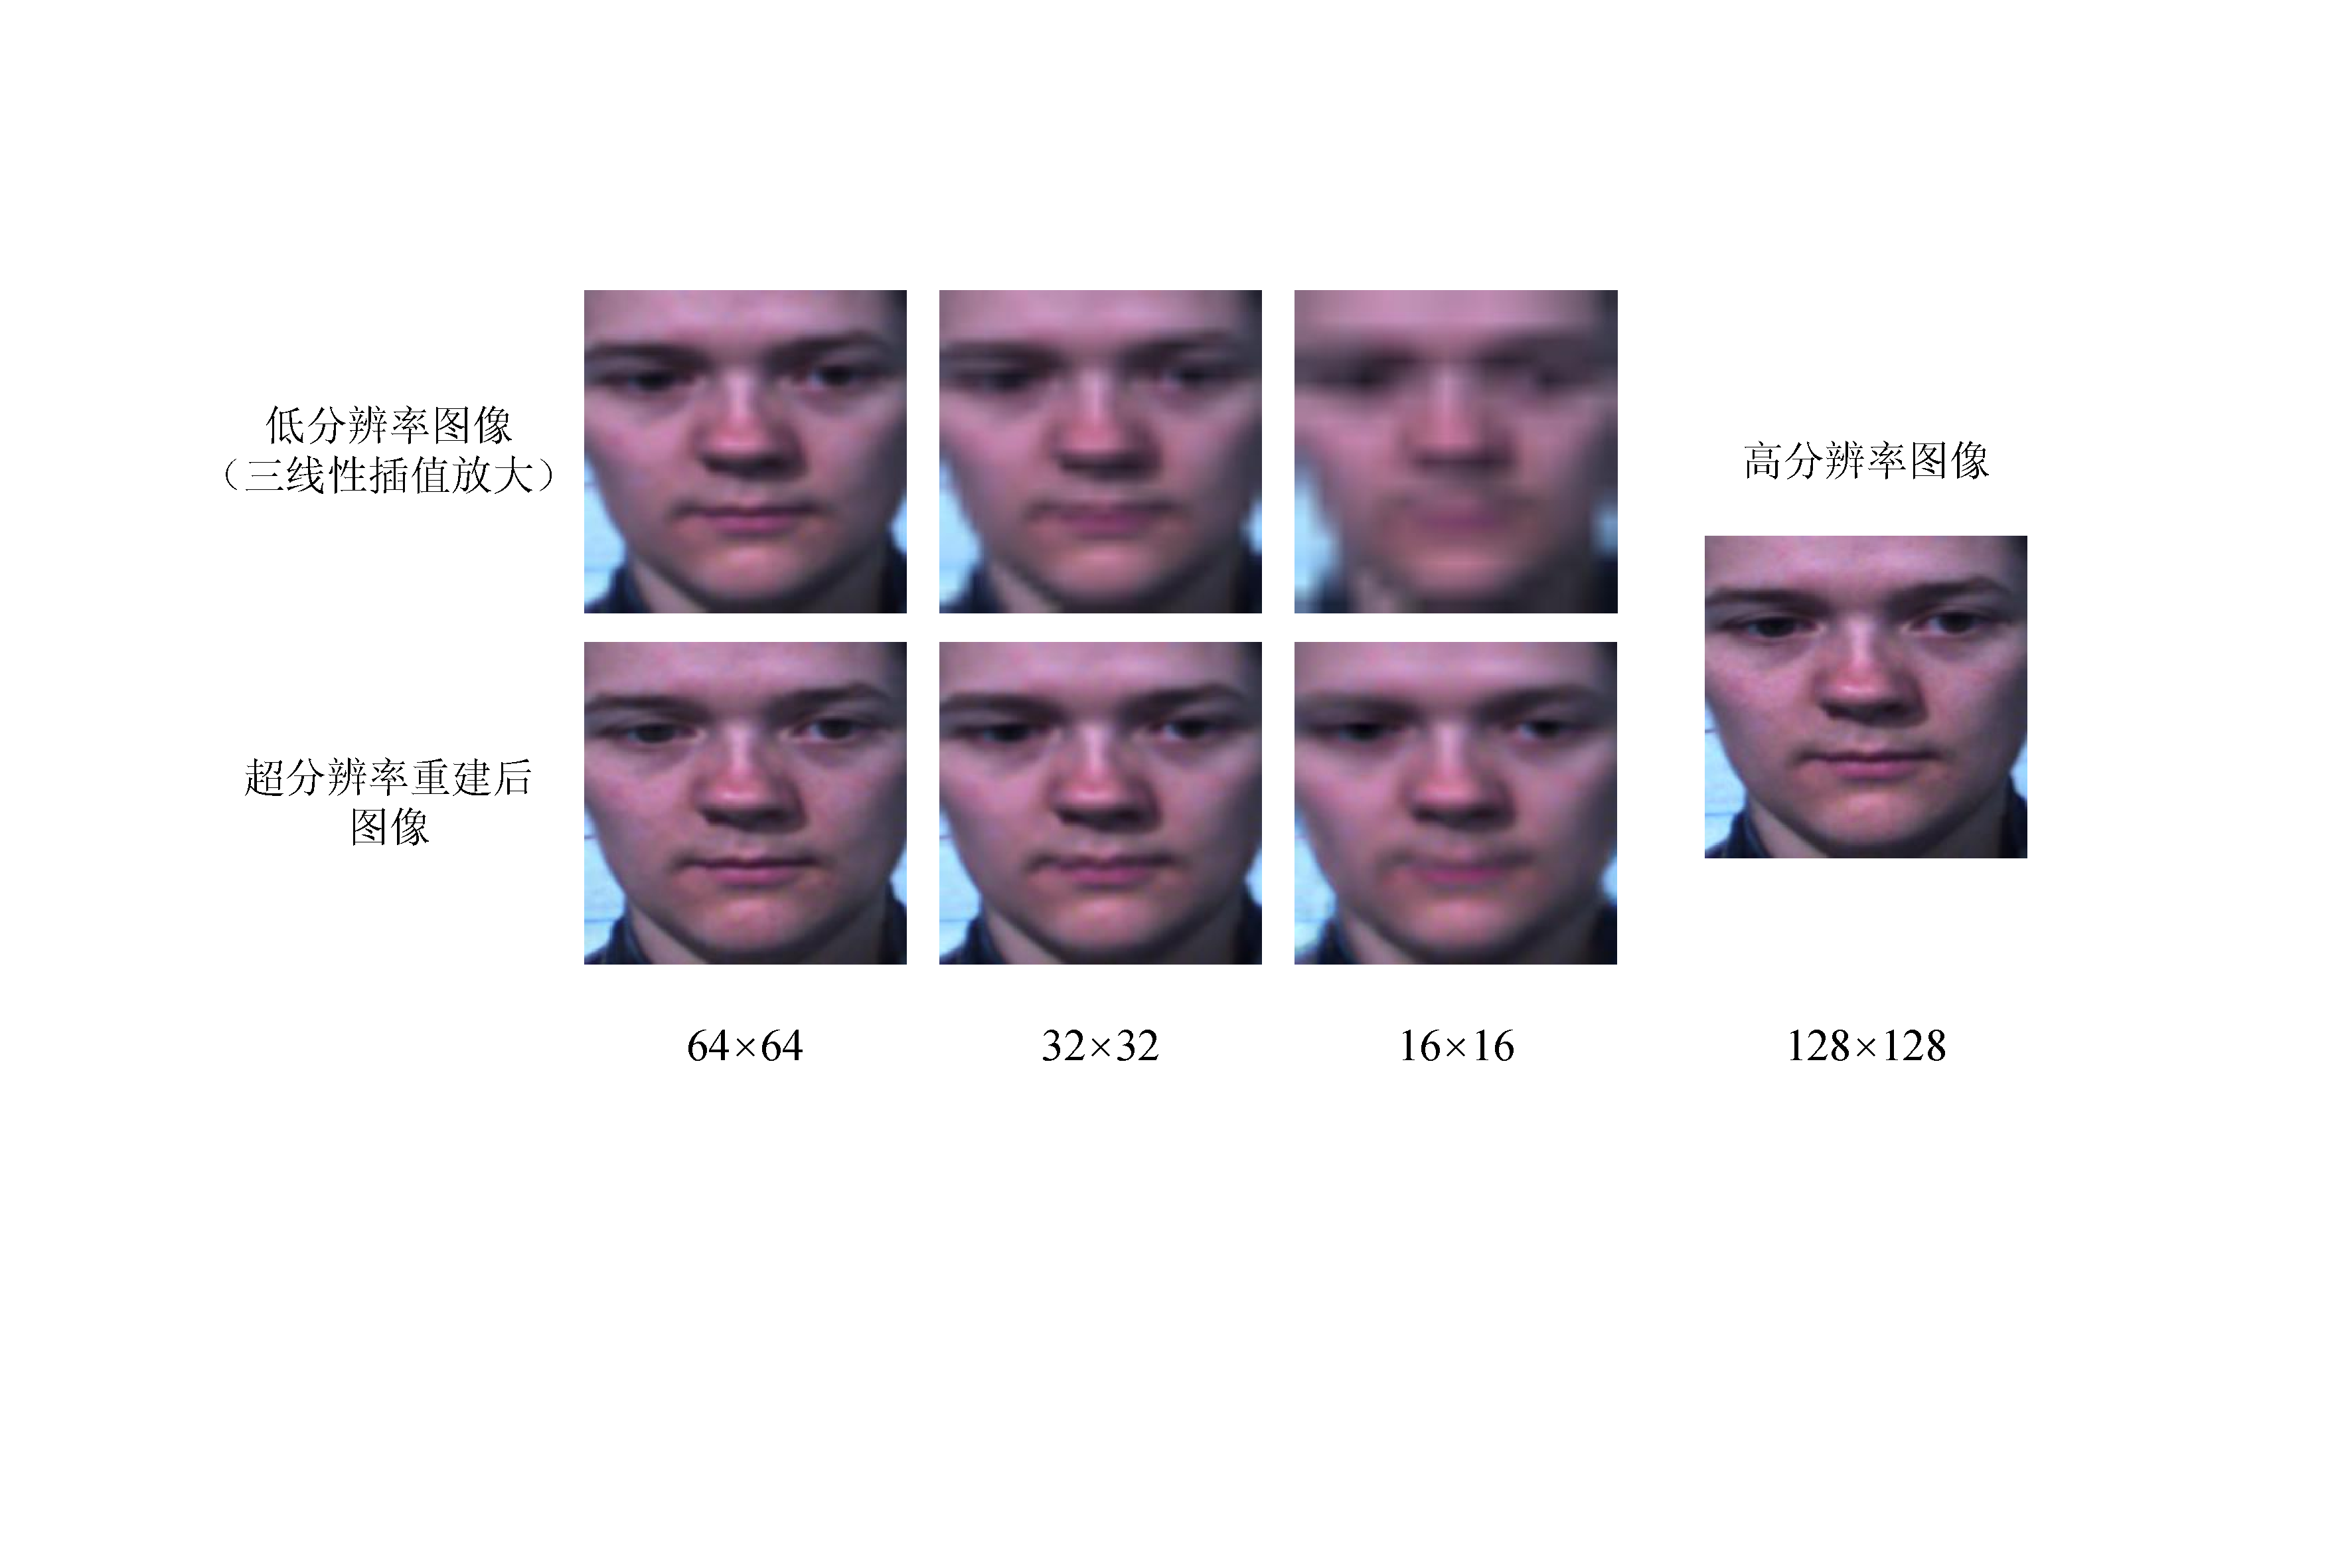
\includegraphics[width=0.75\textwidth]{LR5}
\caption{不同分辨率图像重建结果比较}
\label{fig15}
\end{figure}

为了对视频片段的时长进行归一化,使用TIM算法将视频片段的帧数插值为10帧,如2.2节所述。我们应用快速LBP-TOP将视频剪辑成不同的长方体和提取每个长方体的LBP-TOP特征构成一个完整的功能,使用统一的映射,半径设置为$ r=2 $,和相邻点$p$的数量设置为$ p=8 $。我们使用leave-one-subject-out协议进行实验,即,将一个受试者的所有样本作为测试集,其他受试者的所有样本作为训练集。我们采用LSVM作为分类器,其中惩罚系数$c=1$。

在本节中,我们提出了低分辨率图像序列的微表情识别性能的基线。为了适应不同分辨率的测试样本,我们将训练集从$ 128 \times 128 $下采样到对应的分辨率(即),以便进行分类程序。注意,下采样操作导致微表达式缺乏判别特征。接下来的实验也表明,在非常低的分辨率下,识别的准确率会急剧下降。

图8显示了不同分辨率图像序列在不同数据集上的识别精度。在这里,我们分别使用L64、L32和L16来命名低分辨率图像序列。从图8可以看出,当输入图像序列的分辨率从$ 64 \times 64 $降低到$ 32 \times 32 $时,SMIC-SubHS数据集(蓝色折线)的识别准确率显著降低。同时,我们可以看到低分辨率图像序列(如L16)的准确率相对较低。这一现象表明,低分辨率的图像序列很难获得满意的结果。主要原因是低分辨率导致微表情描述缺乏高频信息和纹理细节。

\begin{figure}[!htbp]
\centering
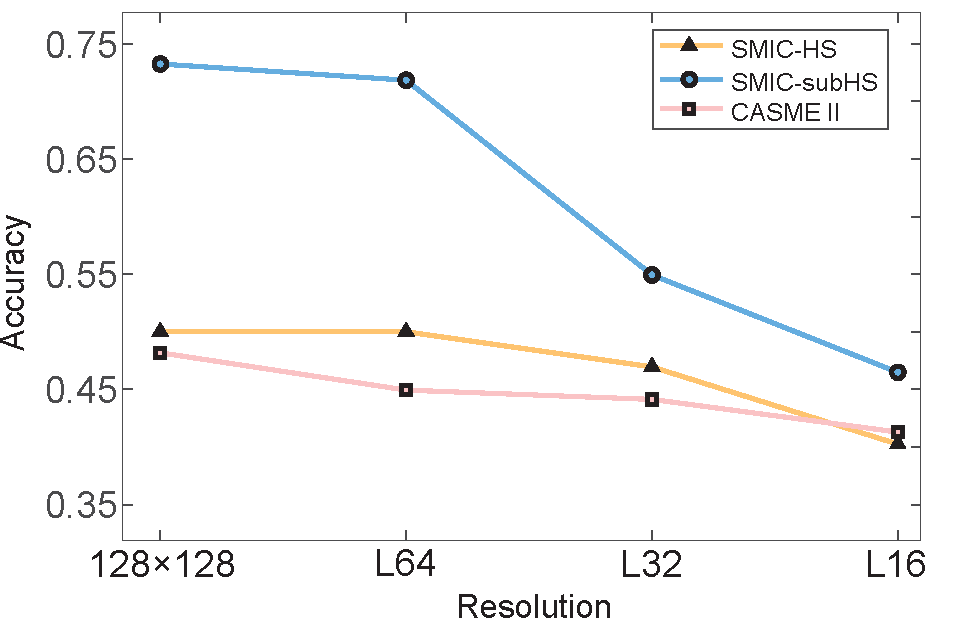
\includegraphics[width=0.60\textwidth]{LR6}
\caption{不同数据集不同分辨率的图像序列的识别准确度}
\label{fig16}
\end{figure}

图9为低分辨率图像序列分类结果的混淆矩阵,并以$ 128 \times 128 $分辨率下的性能为参考。我们可以发现,在SMICSubHS数据集(图9第二列)中,当图像序列的分辨率为$ 128 \times 128 $时,混淆矩阵更加集中在对角线上,说明微表情识别方法的识别效果较好。然而,当图像序列的分辨率降低时,混淆矩阵逐渐变差。我们还可以发现,在SMICHS(图9第一列)和CASME II(图9第三列)中,误分类的比例大于SMICsubHS,图8所示的识别准确率也相对较低。对于SMIC-HS来说,上述问题的主要原因可能是后8个受试者(SMIC-subHS数据集)的分布比前8个受试者更加均衡。对于CASME II来说,主要是由于分布不平衡和类别过多。例如,在CASME II数据集中,来自类other的视频片段数量占40.08\%。

\begin{figure}[]
\centering
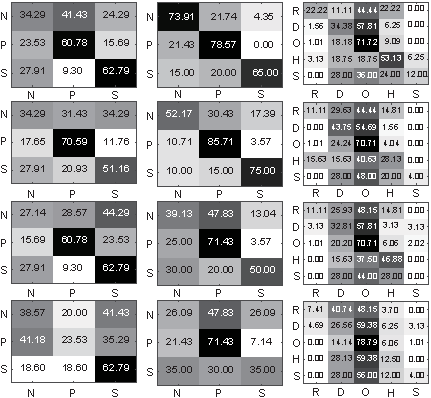
\includegraphics[width=0.75\textwidth]{LR7}
\caption{不同分辨率图像序列的识别准确度混淆矩阵}
\label{fig17}
\end{figure}

水平方向,从左往右依次是SMIC-HS数据集、SMIC-subHS数据集和CASME II数据集。垂直方向,从上到下依次是$ 128 \times 128 $分辨率混淆矩阵、$ 64 \times 64 $分辨率混淆矩阵、$ 32 \times 32 $分辨率混淆矩阵和 $ 16 \times 16 $。其中P代表积极(positive)、N代表消极(negative)、S代表惊喜(surprise)、R代表蔑视(repression)、D代表沮丧(disgust)、O代表其他(others)、H代表开心(happiness)。

在本小节中,我们将在三个数据集上对我们提出的框架进行实验。首先将测试集重构为$ 128 \times 128 $的分辨率,然后在高分辨率空间中进行分类。通过实证分析,选择了最优参数。表4给出了识别精度以及相应的块大小参数设置。从表4可以看出,实验结果有了显著的改善。例如在SMIC-subHS数据集中,$ 64 \times 64 $分辨率下的图像序列识别准确率从71.83\%提高到74.65\%,提高了2.82\%。S32的识别准确率为74.65\%,比L32高19.72\%。S16的识别准确率为73.24\%,比L16高26.76\%。这表明该方法对低分辨率图像序列的微表情识别精度有较好的提高。我们还注意到,与直接将输入作为原始的128128个图像序列相比,该框架使用S64得到了更好的结果。这可能是因为原始SMIC-HS/subHS数据集中的样本在记录过程中存在明显的噪声,使得人脸序列实际上包含了冗余和噪声信息。

超分辨率重建图像序列识别精度的混淆矩阵如图10所示。我们展示了$ 128 \times 128 $、S64、S32和S16图像序列根据不同数据集的识别精度。从图10可以看出,我们提出的框架的混淆矩阵比图9更集中在对角线上。特别是在$ 16 \times 16 $ SMIC-HS数据集(左下),积极的识别精度有显著提高。此外,我们可以从SMIC-subHS数据集(第二列)的结果中看出,将阴性误分类为阳性的比例显著降低,而将阳性正确分类的比例也得到了大幅提高。不幸的是,尽管CASME II数据集(第三列)的结果有所改善,但每个类别的分类仍然很差,通常错误地划分为其他类别。也许是因为其他微表情包含了所有其他类型的微表情,不包括惊讶、快乐、厌恶和压抑,所以它的分类是混合的。综上所述,从图10和图9的对比中我们可以看出,该框架对于低分辨率的微表情识别具有很好的性能提升。

\begin{table}[!htbp]
\centering
\caption{不同分辨率图像在不同数据集上的识别精度比较}
\label{tab7}
\footnotesize% fontsize
\setlength{\tabcolsep}{4pt}% column separation
\renewcommand{\arraystretch}{1.2}%row space
\begin{tabular}{c|c|ccc|ccc}
\hline
\multirow{2}{*}{Accuracy (\%)} & High-resolution & \multicolumn{3}{c|}{Super-resolution Reconstruction} & \multicolumn{3}{c}{Low-resolution} \\ \cline{2-8}
 & $ 128 \times 128 $ & $ 64 \times 64 $ & $ 32 \times 32 $ & $ 16 \times 16 $ & $ 64 \times 64 $ & $ 32 \times 32 $ & $ 16 \times 16 $ \\ \hline
SMIC-HS & \begin{tabular}[c]{@{}c@{}}50.00\\ ($ 8 \times 8 \times 2 $)\end{tabular} & \begin{tabular}[c]{@{}c@{}}52.44\\ ($ 5 \times 5\times 2 $)\end{tabular} & \begin{tabular}[c]{@{}c@{}}51.83\\ ($ 5 \times 5 \times 2 $)\end{tabular} & \begin{tabular}[c]{@{}c@{}}51.83\\ ($ 5 \times 5 \times 2 $)\end{tabular} & \begin{tabular}[c]{@{}c@{}}50.00\\ ($ 6 \times 6 \times 5 $)\end{tabular} & \begin{tabular}[c]{@{}c@{}}46.95\\ ($ 6 \times 6 \times 5 $)\end{tabular} & \begin{tabular}[c]{@{}c@{}}40.24\\ ($ 3 \times 3 \times 6 $)\end{tabular} \\
SMIC-subHS & \begin{tabular}[c]{@{}c@{}}73.24\\ ($ 5 \times 5 \times 2 $)\end{tabular} & \begin{tabular}[c]{@{}c@{}}74.65\\ ($ 5\times 5 \times 2 $)\end{tabular} & \begin{tabular}[c]{@{}c@{}}74.65\\ ($ 5 \times 5 \times 2 $)\end{tabular} & \begin{tabular}[c]{@{}c@{}}73.24\\ ($ 8 \times 8 \times 3 $)\end{tabular} & \begin{tabular}[c]{@{}c@{}}71.83\\ ($ 6 \times 6 \times 2 $)\end{tabular} & \begin{tabular}[c]{@{}c@{}}54.93\\ ($ 6 \times 6 \times 2 $)\end{tabular} & \begin{tabular}[c]{@{}c@{}}46.48\\ ($ 4 \times 4 \times 1 $)\end{tabular} \\
CASME II & \begin{tabular}[c]{@{}c@{}}48.18\\ ($ 7 \times 7 \times 3 $)\end{tabular} & \begin{tabular}[c]{@{}c@{}}48.18\\ ($ 7 \times 7 \times 5 $)\end{tabular} & \begin{tabular}[c]{@{}c@{}}44.53\\ ($ 7 \times 7 \times 3 $)\end{tabular} & \begin{tabular}[c]{@{}c@{}}42.92\\ ($ 7 \times 7 \times 5 $)\end{tabular} & \begin{tabular}[c]{@{}c@{}}44.94\\ ($ 7 \times 7 \times 1 $)\end{tabular} & \begin{tabular}[c]{@{}c@{}}44.13\\ ($ 4 \times 4 \times 2 $)\end{tabular} & \begin{tabular}[c]{@{}c@{}}41.30\\ ($ 2 \times 2 \times 5 $)\end{tabular} \\ \hline
\end{tabular}
\end{table}

High-resolution是指分辨率为$ 128 \times 128 $的图像序列,Super-resolution Reconstruction是指将低分辨率图像序列通过超分辨率重建方法为$ 128 \times 128 $,Low-resolution是指重建前的低分辨率图像序列。$ \mathrm{X} \times \mathrm{Y}  \times \mathrm{T} $指水平、垂直和时间方向块的数量。

本文对低分辨率微表情识别问题进行了全面的研究。我们使用模糊和下采样模型来生成和模拟低分辨率的微表情人脸图像序列。我们在每一帧上使用面部幻觉的方法重建高质量的面部图像序列,增强局部细节,将低质量的图像序列放大到高分辨率的图像序列。然后利用快速LBP-TOP提取动态特征,利用SVM分类器对微表情进行识别。实验结果表明,在低分辨率的微表情识别问题上,该框架在可公开获取的微表情数据集(SMIC-HS、SMIC-subHS、CASME II)上表现良好。未来,我们将重点研究低分辨率情况下微表情识别的深度特征。
